%%%%%%%%%%%%%%%%%%%%%%%%%%%%%%%%%%%%%%%%%%%%%%%%%%%%%%%%%%%%%%%%%%%%%%%%%%%%%%%%%%%%%%%%%%%%%%%%%%%
% Chapter 5 -> Results
% Author: Eduardo G Gusmao
%%%%%%%%%%%%%%%%%%%%%%%%%%%%%%%%%%%%%%%%%%%%%%%%%%%%%%%%%%%%%%%%%%%%%%%%%%%%%%%%%%%%%%%%%%%%%%%%%%%
\chapter{Results}
\label{cha:results}

\graphicspath{{chapter5/figs/}}

% Introduction
In this chapter we present the results generated by our experimental analysis on computational footprinting methods. First, we performed empirical analyses to determine the best parameters to our computational footprinting methodology HINT (Section~\ref{sec:first.hint.parameter.selection}). Then, we investigated two current major challenges in the area: the selection of an optimal footprint ranking strategy and the correction of DNase-seq sequence cleavage bias (Section~\ref{sec:second.footrank.biascorr}). Afterwards, we present our comprehensive comparative analysis, which includes our method, nine competing methods and four baseline methods (Section~\ref{sec:computational.footprinting.methods.comparison}). Then, we showed an example of post-hoc footprinting analysis -- the \emph{de novo} motif finding (Section~\ref{sec:denovo.motif.finding.footprints}). After, we present two case studies in which our computational footprinting method was applied successfully to unravel key regulatory transcription factors on two different biological experiments (Section~\ref{sec:case.studies}). We also provide an insightful discussion on an unexplored and critical challenge of computational footprinting methods -- the transcription factor binding residence time (Section~\ref{sec:impact.tf.residence.time}). Finally, we close this chapter with a thorough discussion on all results obtained in our analysis of computational footprinting methods (Section~\ref{sec:discussion.5}).

%%%%%%%%%%%%%%%%%%%%%%%%%%%%%%%%%%%%%%%%%%%%%%%%%%%%%%%%%%%%%%%%%%%%%
% Section: HINT Parameter Selection
%%%%%%%%%%%%%%%%%%%%%%%%%%%%%%%%%%%%%%%%%%%%%%%%%%%%%%%%%%%%%%%%%%%%%
\section{HINT Parameter Selection}
\label{sec:first.hint.parameter.selection}

% Introduction
We performed a number of preliminary analyses to find the best parameters for our computational footprinting framework HINT. First, we studied the HMM topology which optimizes the accuracy on identifying correct footprints (Section~\ref{sec:ps.hmm.topology}). Then, we tested a number of different combination of input histone modification data. Such test not only determined the best data input types for our computational method but also provided interesting insights on the underlying biological problem (Section~\ref{sec:ps.combination.histone.modifications}). Finally, we investigated the level of dependence our method has on the training data (Section~\ref{sec:ps.hmm.training}). 

% Overview of the tests
In the analyses presented in this section, we used the ChIP-seq evaluation approach to assess performance. All scenarios were tested with regard to their accuracy on predicting footprints using the AUC at $100\%$ false positive rate (FPR) on the {\tt Comprehensive Dataset}. Since we are evaluating the impact on performance of different data types (DNase-seq, different combinations of histone modifications ChIP-seq and different combinations of both DNase-seq and histone modifications) we opted to use the motif-predicted binding sites' bit-score as the ranking metric to create the ROC curves. The rationale for the usage of such ranking strategy is that it is independent of the experimental open chromatin datasets. This is necessary because: (1) this ranking strategy does not bias the analysis towards specific HMM topologies/input data type and (2) it makes the analysis interpretation simpler. In this scenario, we divided the gold standard data set into two groups: the motif-predicted binding sites that contain at least one bp overlap with HINT's predicted footprints and the ones that do not overlap. Both groups were sorted based on the motif matching bit-score. A single list is then obtained by combining the ranked list of predicted sites before the ranked list of the non-predicted sites. The ROC curve is created based on this combined ranked list of motif-predicted binding sites. These analyses were performed using data from chromosome 1 only, which was removed from the comparative analyses (in Section~\ref{sec:computational.footprinting.methods.comparison}) to allow a fair comparison.

%%%%%%%%%%%%%%%%%%%%%%%%%%%%%%%%%%%%%%%%%%%%%%%%%%%%%%%%%%%%%%%%%%%%%
% Section: HMM Topology
%%%%%%%%%%%%%%%%%%%%%%%%%%%%%%%%%%%%%%%%%%%%%%%%%%%%%%%%%%%%%%%%%%%%%
\subsection{HMM Topology}
\label{sec:ps.hmm.topology}

% Introduction
We investigated the different HMM topologies presented in this thesis (see Section~\ref{sec:hmm.topology}). The empirical test consists on evaluating the area under the ROC curve (AUC) using the {\tt Comprehensive Dataset} from the ChIP-seq evaluation approach. The distribution of the $233$ AUCs at $100\%$ false positive rate (one for each transcription factor from the {\tt Comprehensive Dataset}) for all the HMM topologies can be seen in Figure~\ref{fig:gusmao_HINT_topologies}. All the HMM topologies that use histone modification data were tested using a combination of H3K4me1 $+$ H3K4me3.

% First glance
We are able to observe in Figure~\ref{fig:gusmao_HINT_topologies} that the original DNase+histone provides higher accuracies than all other models. Furthermore, the histone-only HMM provides the lowest accuracies. This relates to the fact that the histone-only footprints are large and do not capture the spatial specificity provided by the higher-resolution DNase-seq data.

% Figure - Performance of different HINT HMM topologies
\begin{figure}[h!]
\centering
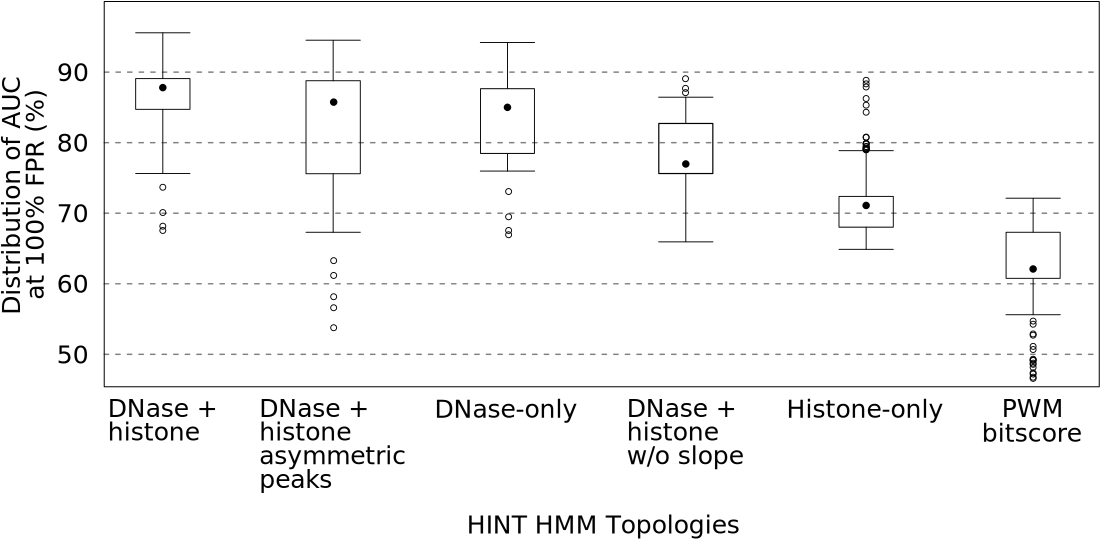
\includegraphics[width=0.9\textwidth]{gusmao_HINT_topologies}
\caption[Performance of different HINT HMM topologies]{\textbf{Performance of different HINT HMM topologies.} Distribution of AUC at $100\%$ false positive rate (FPR) of the ROC curves generated using the ChIP-seq evaluation {\tt Comprehensive Dataset} on different HINT HMM topologies. The histone modification combination H3K4me1 $+$ H3K4me3 was used on the HMM topologies which use such data.}
\label{fig:gusmao_HINT_topologies}
\end{figure}

% Friedman-Nemenyi
We performed a Friedman-Nemenyi test on the distribution of accuracies from different HMM topologies to assess statistical significance. The results can be seen in Table~\ref{tab:fn_gusmao_HINT_topologies}. We observed that indeed the original DNase+histone model significantly outperforms all other topologies. This analysis shows that the proper integration of DNase-seq and histone modifications results in significantly higher accuracies than using each of these data separately.

% DNase-seq+histone models
The possible reason for the good results of the original DNase+histone topology in relation to the DNase+histone asymmetric peaks topology is the fact that the normalization methodology emphasizes even little increases in histone levels, leveraging the asymmetry issue (see Figure~\ref{fig:gusmao_assymetric_correction}). Furthermore, the poor performance of the DNase+histone without slope topology in comparison to the other DNase+histone topologies indicates that even with more complex models ($4$ \emph{vs} $2$ variables and $8$ \emph{vs} $4$ states, respectively) the slope signal and the additional states are crucial in the accurate delineation of the footprints.

% DNase-only and histone-only
It is interesting to observe that the DNase-only HMM topology provides high accuracies (significantly better than the DNase+histone without slope and histone-only topologies) and is competitive with the original and asymmetric peaks DNase+histone topologies. This fact shows the power of the DNase-seq data on identifying transcription factor footprints. On the other hand, although the histone-only topology presents significantly lower accuracies than all other topologies (median AUC $= 71\%$), it is still a better choice than purely sequence-based approaches (median AUC $= 62\%$).

% Table - Friedman-Nemenyi test on different HINT HMM topologies
\begin{table}[h!]
\footnotesize
\vspace{0.0cm}
\begin{center}
\caption[Friedman-Nemenyi test on different HINT HMM topologies]{\textbf{Friedman-Nemenyi test on different HINT HMM topologies.} Friedman-Nemenyi hypothesis test results on AUC at $100\%$ false positive rate (FPR) of the ROC curves generated using the ChIP-seq evaluation {\tt Benchmarking Dataset} on different HINT HMM topologies. The asterisk and the cross, respectively, indicate that the method in the column outperformed the method in the row with significance levels of 0.01 and 0.05.}
\label{tab:fn_gusmao_HINT_topologies}
\renewcommand{\arraystretch}{1.2}
  \begin{tabular}{ rccccc }
    & \rotatebox{90}{DNase$+$histone} & \rotatebox{90}{\specialcell{DNase$+$histone \\[-0.3cm] asymmetric}} & \rotatebox{90}{DNase-only} & \rotatebox{90}{\specialcell{DNase$+$histone \\[-0.3cm] w/o slope}} & \rotatebox{90}{Histone-only} \\
    \hline
    DNase$+$histone &  &  &  &  &   \\
    DNase$+$histone asymmetric & $*$ &  &  &  &  \\
    DNase-only & $*$ &  &  &  &  \\
    DNase$+$histone w/o slope & $*$ & $*$ & $*$ &  &  \\
    Histone-only &$*$  & $*$ & $*$ & $*$  & \\
    \hline
  \end{tabular}
\end{center}
\vspace{0.0cm}
\end{table}

% Figure - Histone asymmetry example
\begin{figure}[h!]
\centering
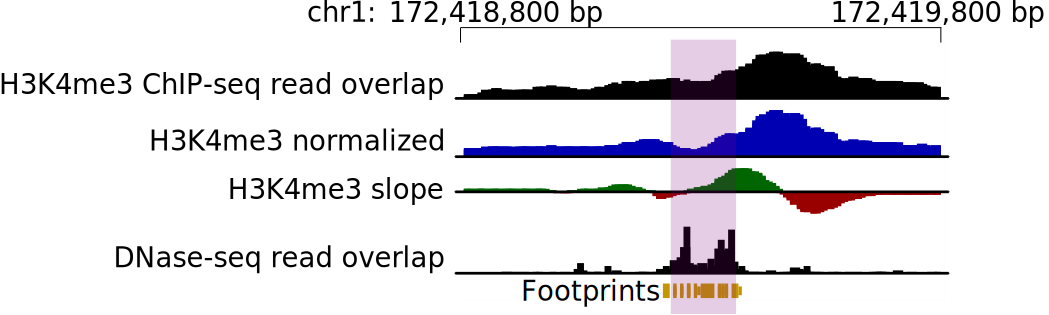
\includegraphics[width=0.9\textwidth]{gusmao_assymetric_correction}
\caption[Histone asymmetry example]{\textbf{Histone asymmetry example.} H3K4me3 ChIP-seq raw count (top black), normalized (blue) and slope (green for positive and red for negative) signals; DNase-seq count signal (bottom black) and footprints (yellow) predicted in a region with asymmetrical histone modification profile. Although the leftmost peak from the peak-dip-peak pattern of the H3K4me3 contains very small count signals (very close to the background signal, in this region), original DNase+histone HINT topology is still capable of predicting the footprints within the DHS region. Note that after the normalization of the H3K4me3 counts, the resulting signal delineates the DHS region more clearly (depicted by the purple box).}
\label{fig:gusmao_assymetric_correction}
\end{figure}

%%%%%%%%%%%%%%%%%%%%%%%%%%%%%%%%%%%%%%%%%%%%%%%%%%%%%%%%%%%%%%%%%%%%%
% Section: Combination of Histone Modifications
%%%%%%%%%%%%%%%%%%%%%%%%%%%%%%%%%%%%%%%%%%%%%%%%%%%%%%%%%%%%%%%%%%%%%
\subsection{Combination of Histone Modifications}
\label{sec:ps.combination.histone.modifications}

% Introduction
We have performed an empirical test on the predictive power of combining different histone modifications using HINT's original DNase+histone HMM topology. In this test we considered the histone modifications H3K4me1, H3K4me3, H3K9ac, H3K27ac and the histone variant H2A.Z (referred to with the term ``histone modification'', for simplicity of notation). The presence of such histones modifications are associated with active regulatory regions. We compared the performance using each of these histone modifications individually ($5$ prediction sets, one for each histone modification). We also evaluated the combination of all pairs and triples of histone signals by simply merging all predicted sites (as described in Section~\ref{sec:hint.application}). Such combinatorial analysis generates $20$ additional prediction sets ($10$ pairs and $10$ triples). Note that extending to further combinations would deviate from one of the main goals of this study, which is to create a consistent map of active transcription factor binding sites with few genome-wide assays. We tested all the $25$ combinations using the ChIP-seq evaluation {\tt Comprehensive Dataset} gold standard.

% Figure and FN overall
The Figure~\ref{fig:gusmao_HINT_histones} presents the distribution of AUCs for all histone modification models tested plus the DNase-only HMM topology for comparison purpose. We observed that most methods presented the region between the first and third quartiles approximately between AUCs $80\%$--$95\%$. In order to test the statistical relevance of these differences, we performed a Friedman-Nemenyi test. The Table~\ref{tab:fn_gusmao_HINT_histones} shows the accuracy ranking for all histone modification combinations in decreasing order, providing information on which models significantly outperformed others.

% Result
Overall, results indicate that combinations with more histone marks are better than single-histone models. Several combinations of three marks (H3K4me1+H3K4me3+H3K9ac, H3K4me1+H3K4me3+H3K27ac, H2A.Z+H3K4me1+H3K4me3, H2A.Z+H3K4me3+H3K9ac and H3K4me3+H3K9ac+H3K27ac) were similarly good, i.e. their AUC are not significantly lower than any other combination. Similarly, if we only consider individual and pairs of histone marks, H3K4me1+H3K4me3, H3K4me3+H3K9ac, H3K4me3+H3K27ac, H2A.Z+H3K4me3 and H3K4me1+H3K9ac have similar AUCs. This indicates that any combination of these histone marks, whenever available, would perform equally well. Nevertheless, we observed that the DNase-only topology outperforms a few DNase+histone modification combinations significantly. This represents further evidence of the importance of such high-resolution signal and might explain previous failed attempts to improve the accuracy of transcription factor predictions by introducing histone modifications individually~\cite{pique2011,cuellar2012}.

% Figure - Performance of different histone modification combinations
\begin{figure}[h!]
\centering
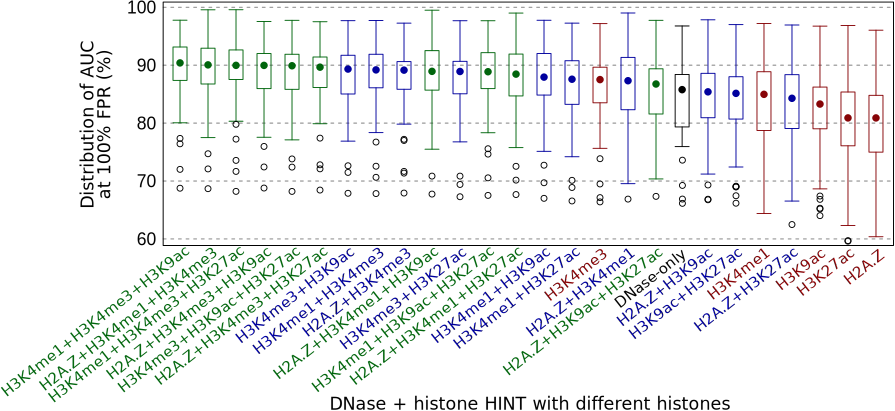
\includegraphics[width=0.95\textwidth]{gusmao_HINT_histones}
\caption[Performance of different histone modification combinations]{\textbf{Performance of different histone modification combinations.} Distribution of AUC at $100\%$ false positive rate (FPR) of the ROC curves generated using the ChIP-seq evaluation {\tt Benchmarking Dataset} on DNase + histone HINT topology with different combinations of histone modifications. We show single, pairs and trios of histone modifications in red, blue and green, respectively. The DNase-only accuracy is also shown (in black) for comparison purpose.}
\label{fig:gusmao_HINT_histones}
\end{figure}

% Table - Friedman-Nemenyi test on different histone modification combinations
\begin{table}[h!]
\scriptsize
\vspace{0.0cm}
\begin{center}
\caption[Friedman-Nemenyi test on different histone modification combinations]{\textbf{Friedman-Nemenyi test on different histone modification combinations.} Friedman-Nemenyi hypothesis test results on AUC at $100\%$ false positive rate (FPR) of the ROC curves generated using the ChIP-seq evaluation {\tt Benchmarking Dataset} on DNase + histone HINT topology with different combinations of histone modifications. We show single, pairs and trios of histone modifications in shades of red, blue and green, respectively. In addition, we also show the DNase-only HMM topology for comparison purpose (gray). The asterisk and the cross, respectively, indicate that the method in the column outperformed the method in the row with significance levels of 0.01 and 0.05.}
\label{tab:fn_gusmao_HINT_histones}
\renewcommand{\arraystretch}{1.2}
\setlength{\tabcolsep}{3pt}
  \begin{tabular}{ rABABABCABCACDCDCAEGCDECEFE }
    & \rotatebox{90}{H3K4me1+H3K4me3+H3K9ac} & \rotatebox{90}{H3K4me1+H3K4me3+H3K27ac} & \rotatebox{90}{H2A.Z+H3K4me1+H3K4me3} & \rotatebox{90}{H2A.Z+H3K4me3+H3K9ac} & \rotatebox{90}{H3K4me3+H3K9ac+H3K27ac} & \rotatebox{90}{H2A.Z+H3K4me3+H3K27ac} & \rotatebox{90}{H3K4me1+H3K4me3} & \rotatebox{90}{H3K4me1+H3K9ac+H3K27ac} & \rotatebox{90}{H2A.Z+H3K4me1+H3K9ac} & \rotatebox{90}{H3K4me3+H3K9ac} & \rotatebox{90}{H2A.Z+H3K4me1+H3K27ac} & \rotatebox{90}{H3K4me3+H3K27ac} & \rotatebox{90}{H2A.Z+H3K4me3} & \rotatebox{90}{H3K4me1+H3K9ac} & \rotatebox{90}{H3K4me1+H3K27ac} & \rotatebox{90}{H2A.Z+H3K4me1} & \rotatebox{90}{H2A.Z+H3K9ac+H3K27ac} & \rotatebox{90}{H3K4me3} & \rotatebox{90}{DNase-only} & \rotatebox{90}{H2A.Z+H3K9ac} & \rotatebox{90}{H3K9ac+H3K27ac} & \rotatebox{90}{H3K4me1} & \rotatebox{90}{H2A.Z+H3K27ac} & \rotatebox{90}{H3K9ac} & \rotatebox{90}{H3K27ac} & \rotatebox{90}{H2A.Z} \\
    \hline
    H3K4me1+H3K4me3+H3K9ac &     &     &     &     &     &     &     &     &     &     &     &     &     &     &     &     &     &     &     &     &     &     &     &     &     &      \\
    H3K4me1+H3K4me3+H3K27ac &     &     &     &     &     &     &     &     &     &     &     &     &     &     &     &     &     &     &     &     &     &     &     &     &      &     \\
    H2A.Z+H3K4me1+H3K4me3 &     &     &     &     &     &     &     &     &     &     &     &     &     &     &     &     &     &     &     &     &     &     &     &     &     &      \\
    H2A.Z+H3K4me3+H3K9ac &     &     &     &     &     &     &     &     &     &     &     &     &     &     &     &     &     &     &     &     &     &     &     &     &      &     \\
    H3K4me3+H3K9ac+H3K27ac &     &     &     &     &     &     &     &     &     &     &     &     &     &     &     &     &     &     &     &     &     &     &     &     &      &     \\
    H2A.Z+H3K4me3+H3K27ac & $*$ &     &     &     &     &     &     &     &     &     &     &     &     &     &     &     &     &     &     &     &     &     &     &     &      &     \\
    H3K4me1+H3K4me3 & $*$ &     &     &     &     &     &     &     &     &     &     &     &     &     &     &     &     &     &     &     &     &     &     &     &     &      \\
    H3K4me1+H3K9ac+H3K27ac & $*$ & $+$ &     &     &     &     &     &     &     &     &     &     &     &     &     &     &     &     &     &     &     &     &     &     &      &     \\
    H2A.Z+H3K4me1+H3K9ac & $*$ & $*$ & $*$ &     &     &     &     &     &     &     &     &     &     &     &     &     &     &     &     &     &     &     &     &     &     &      \\
    H3K4me3+H3K9ac & $*$ & $*$ & $*$ &     &     &     &     &     &     &     &     &     &     &     &     &     &     &     &     &     &     &     &     &     &      &     \\
    H2A.Z+H3K4me1+H3K27ac & $*$ & $*$ & $*$ & $*$ & $+$ &     &     &     &     &     &     &     &     &     &     &     &     &     &     &     &     &     &     &     &      &     \\
    H3K4me3+H3K27ac & $*$ & $*$ & $*$ & $*$ & $*$ &     &     &     &     &     &     &     &     &     &     &     &     &     &     &     &     &     &     &     &      &     \\
    H2A.Z+H3K4me3 & $*$ & $*$ & $*$ & $*$ & $*$ &     &     &     &     &     &     &     &     &     &     &     &     &     &     &     &     &     &     &     &      &     \\
    H3K4me1+H3K9ac & $*$ & $*$ & $*$ & $*$ & $*$ & $*$ &     &     &     &     &     &     &     &     &     &     &     &     &     &     &     &     &     &     &      &     \\
    H3K4me1+H3K27ac & $*$ & $*$ & $*$ & $*$ & $*$ & $*$ & $*$ & $*$ & $*$ & $*$ &     &     &     &     &     &     &     &     &     &     &     &     &     &     &      &     \\
    H2A.Z+H3K4me1 & $*$ & $*$ & $*$ & $*$ & $*$ & $*$ & $*$ & $*$ & $*$ & $*$ & $*$ & $*$ &     &     &     &     &     &     &     &     &     &     &     &     &      &     \\
    H2A.Z+H3K9ac+H3K27ac & $*$ & $*$ & $*$ & $*$ & $*$ & $*$ & $*$ & $*$ & $*$ & $*$ & $*$ & $*$ & $*$ &     &     &     &     &     &     &     &     &     &     &     &     &      \\
    H3K4me3 & $*$ & $*$ & $*$ & $*$ & $*$ & $*$ & $*$ & $*$ & $*$ & $*$ & $*$ & $*$ & $*$ & $*$ &     &     &     &     &     &     &     &     &     &     &     &      \\

    DNase-only & $*$ & $*$ & $*$ & $*$ & $*$ & $*$ & $*$ & $*$ & $*$ & $*$ & $*$ & $*$ & $*$ & $*$ & $*$ &     &     &     &     &      &     &     &     &     &    &      \\

    H2A.Z+H3K9ac & $*$ & $*$ & $*$ & $*$ & $*$ & $*$ & $*$ & $*$ & $*$ & $*$ & $*$ & $*$ & $*$ & $*$ & $*$ &     &     &     &     &      &     &     &     &     &     &     \\
    H3K9ac+H3K27ac & $*$ & $*$ & $*$ & $*$ & $*$ & $*$ & $*$ & $*$ & $*$ & $*$ & $*$ & $*$ & $*$ & $*$ & $*$ &     &     &     &    &      &     &     &     &     &      &    \\
    H3K4me1 & $*$ & $*$ & $*$ & $*$ & $*$ & $*$ & $*$ & $*$ & $*$ & $*$ & $*$ & $*$ & $*$ & $*$ & $*$ & $*$ & $*$ &     &     &     &     &     &     &     &     &     \\
    H2A.Z+H3K27ac & $*$ & $*$ & $*$ & $*$ & $*$ & $*$ & $*$ & $*$ & $*$ & $*$ & $*$ & $*$ & $*$ & $*$ & $*$ & $*$ & $*$ & $+$ &  $+$  &      &     &     &     &     &     &     \\
    H3K9ac & $*$ & $*$ & $*$ & $*$ & $*$ & $*$ & $*$ & $*$ & $*$ & $*$ & $*$ & $*$ & $*$ & $*$ & $*$ & $*$ & $*$ & $*$ &  $*$  &      &     &     &     &     &     &     \\
    H3K27ac & $*$ & $*$ & $*$ & $*$ & $*$ & $*$ & $*$ & $*$ & $*$ & $*$ & $*$ & $*$ & $*$ & $*$ & $*$ & $*$ & $*$ & $*$ & $*$ & $*$ &  $*$ &   &     &     &    &     \\
    H2A.Z & $*$ & $*$ & $*$ & $*$ & $*$ & $*$ & $*$ & $*$ & $*$ & $*$ & $*$ & $*$ & $*$ & $*$ & $*$ & $*$ & $*$ & $*$ & $*$ & $*$ &  $*$ &   &     &     &     &    \\
    \hline
  \end{tabular}
\end{center}
\vspace{0.0cm}
\end{table}

%%%%%%%%%%%%%%%%%%%%%%%%%%%%%%%%%%%%%%%%%%%%%%%%%%%%%%%%%%%%%%%%%%%%%
% Section: HMM Training
%%%%%%%%%%%%%%%%%%%%%%%%%%%%%%%%%%%%%%%%%%%%%%%%%%%%%%%%%%%%%%%%%%%%%
\subsection{HMM Training}
\label{sec:ps.hmm.training}

% Introduction
The annotation of certain genomic regions with the HMM states in order to train HINT is laborious. Therefore, we decided to analyze whether HINT's performance is impacted by training and applying the method to data from different cell types. In this particular empirical test, we used {\tt Comprehensive Dataset}'s evaluation data for four cell types: H1-hESC ($29$ TFs), HeLa-S3 ($20$ TFs), HepG2 ($21$ TFs) and K562 ($59$ TFs).

% The test
We have compared the AUC values of HINT when it was trained in a particular cell type and executed in the same cell type it was trained \emph{vs} the other three cell types. The Friedman-Nemenyi test was applied to assess statistical significance.

% Figure
The Figure~\ref{fig:gusmao_HINT_training} shows the results for all models applied to all cell types tested. Each set of four boxplots represent one of the four HINT models (trained with data from one of the four cell types), which was applied to the signal generated from the cell type labeled on the bottom of the set. Statistical significance are directly represented in the graph.

% Results
We can observe in Figure~\ref{fig:gusmao_HINT_training} that only in one out of twelve cases the AUC levels are significantly different ($p$-value $< 0.05$). This corresponds to the HepG2 model, when used to generate footprints in the same cell type and in K562 cell type. These results suggest that our signal processing workflow and HMM model are able to robustly mitigate differences between distinct cell type signals. Consequently, we can consider HINT cell-type training-independent. The practical implication of such an important characteristic is that a simple application of a model already stored in our software tool, trained for a particular cell type, is sufficient to generate accurate predictions for any other cell type, without the need to re-train the model. Furthermore, this is evidence that the patterns that make the grammar of active TFBSs are similar between different cells.

% Figure - Performance of different HMM training/testing scenarios
\begin{figure}[h!]
\centering
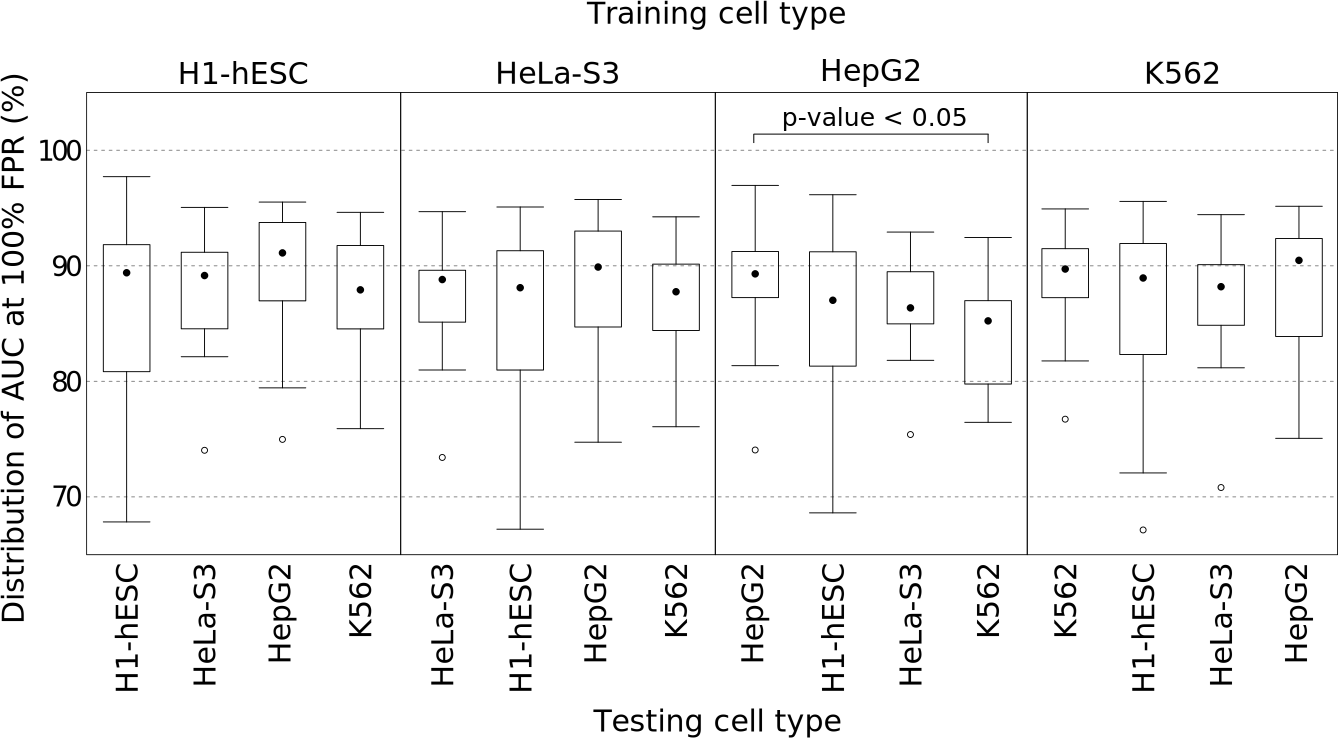
\includegraphics[width=0.99\textwidth]{gusmao_HINT_training}
\caption[Performance of different HMM training/testing scenarios]{\textbf{Performance of different HMM training/testing scenarios.} Distribution of AUC at $100\%$ false positive rate (FPR) of the ROC curves generated using the ChIP-seq evaluation {\tt Benchmarking Dataset} on HINT models trained in four different cell types (top $x$-axis labels) and applied to (tested on) the same four cell types (bottom $x$-axis labels). The first boxplot within each set represents the model trained in the same cell type as the one it was applied to. Statistical significance on the pairwise difference between these distributions is represented by the three-star system.}
\label{fig:gusmao_HINT_training}
\end{figure}

%%%%%%%%%%%%%%%%%%%%%%%%%%%%%%%%%%%%%%%%%%%%%%%%%%%%%%%%%%%%%%%%%%%%%
% Section: Footprint Scoring and Sequence Cleavage Bias Correction
%%%%%%%%%%%%%%%%%%%%%%%%%%%%%%%%%%%%%%%%%%%%%%%%%%%%%%%%%%%%%%%%%%%%%
\section{Footprint Scoring and Sequence Cleavage Bias Correction}
\label{sec:second.footrank.biascorr}

% Introduction
In this section we focused on two important challenges regarding computational footprinting methods. First, we performed a series of empirical tests on HINT and competing methods to identify an optimal footprinting scoring metric (Section~\ref{sec:footprint.ranking.strategy}). We investigated such optimal scoring metric for both evaluation methodologies proposed (ChIP-seq and gene expression). Second, we investigated the impact of the DNase-seq sequence cleavage bias on computational footprinting and whether such bias could be corrected to improve the performance of HINT (Section~\ref{sec:impact.dnase.sequence.cleavage.bias}). All DNase-seq sequence cleavage bias analyses used the ChIP-seq evaluation strategy, since we require the transcription factor-wise results provided by this evaluation strategy.

% Overview of the tests
Regarding the ChIP-seq evaluation analyses presented in this section; since such experiments required a few comparisons between HINT and other competing methods which only used DNase-seq data as input, we opted to use the DNase-only HMM topology to provide a fairer comparison. In analyses that involved HINT and competing methods we used the {\tt Benchmarking Dataset} as gold standard; while in analyses that involved only HINT we used the full {\tt Comprehensive Dataset}. Furthermore, we decided to use the AUC at $10\%$ FPR to capture more subtle differences in reported accuracies. These analyses were performed using data from chromosome 1 only, which was removed from the comparative analyses (in Section~\ref{sec:computational.footprinting.methods.comparison}) to allow a fair comparison.

%%%%%%%%%%%%%%%%%%%%%%%%%%%%%%%%%%%%%%%%%%%%%%%%%%%%%%%%%%%%%%%%%%%%%
% Section: Footprint Ranking Strategy
%%%%%%%%%%%%%%%%%%%%%%%%%%%%%%%%%%%%%%%%%%%%%%%%%%%%%%%%%%%%%%%%%%%%%
\subsection{Footprint Ranking Strategy}
\label{sec:footprint.ranking.strategy}

% Introduction
Some competing footprinting methods also provide statistics to rank footprint predictions. Wellington and DNase2TF use read count statistics to provide $p$-values for each footprint. Several site-centric approaches provide either probabilities (BinDNase, Centipede and PIQ) or log-odds scores (FLR) of footprints. Other methods use statistics such as FS (Neph) or PWM bit-score (Cuellar), to rank predicted footprints.

% Introduction
The main goal of this empirical analysis is to identify the best scoring metric for footprint predictions. For that, we used the transcription factor-wise ChIP-seq evaluation approach to search for such scoring metric by performing an empirical test on the accuracy of HINT and competing methods (Section~\ref{sec:frs.chipseq.evaluation}). Since the gene expression evaluation differs in nature with regard to the scoring metric (footprint quality score), we also evaluated the best scoring metric using such evaluation approach (Section~\ref{sec:frs.gene.expression.evaluation}).

% Section: ChIP-seq Evaluation
\subsubsection{ChIP-seq Evaluation}
\label{sec:frs.chipseq.evaluation}

% Introduction
The ChIP-seq evaluation scheme requires a metric to rank the footprint predictions. Since the ChIP-seq evaluation scheme is evaluated in a transcription factor-wise manner, we can regard an optimal ranking score to create the ROC curve as the best footprint ranking scheme.

% The test
We investigated three footprint scoring metrics: the tag count (TC), footprint score (FS) and the PWM bit-score (PWM). We assigned a quality score for each footprint predicted using the DNase-only HINT method. The assignment of the TC and FS to each footprint can be performed straightforwardly using the DNase-seq data. Regarding the PWM metric, each footprint was assigned to the bit-score of its overlapping motif-predicted binding site. The PWM score assignment was performed as a ``control'' experiment, since it requires motif-predicted binding sites, which are only available for known transcription factors.

% Figure
The test consists on ranking the footprints by each of these three different metrics and creating the ROC curves based on each different ranking. Figure~\ref{fig:gusmao_HINT_chipseq_rank} shows the distribution of the AUC at $10\%$ FPR for different footprint ranking strategies using HINT's footprint predictions. The statistical significance assessment in the graph corresponds to the Friedman-Nemenyi test.

% Results
We are able to observe that the TC is the best footprint ranking strategy (average AUC $= 90\%$), outperforming both FS and PWM ($p$-value $< 0.01$). Furthermore, it is clear that both FS and PWM have significantly lower accuracies than the TC strategy (average AUC $= 50\%$ and $37\%$, respectively; $p$-value $< 0.01$). It is clear that the PWM bit-score is the worst scoring metric, since it does not use the cell-specific open chromatin information provided by the DNase-seq data. However, the success of the TC metric in comparison to the FS is not so straightforward. The FS is defined as a ratio between the DNase-seq at the center of the footprint and its flanking regions. The first problem that the FS encounters is that it does not recover the absolute signal intensity, as the simpler TC metric does. The second problem of the FS metric regards the window length in which the average signal in the center of the motif and flanking regions are evaluated. This issue is similar to the one discussed for window-based segmentation methods (see Section~\ref{sec:method.definition}). We believe these issues are related to the higher observed accuracies for the TC metric.

% Figure - Performance of different footprint ranking strategies on HINT
\begin{figure}[h!]
\centering
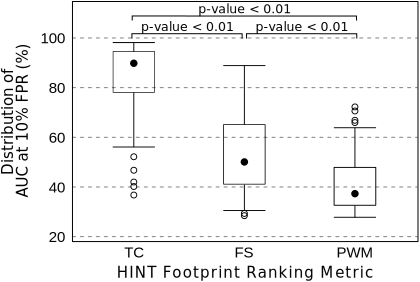
\includegraphics[width=0.5\textwidth]{gusmao_HINT_chipseq_rank}
\caption[Performance of different footprint ranking strategies on HINT]{\textbf{Performance of different footprint ranking strategies on HINT} Distribution of AUC at $10\%$ false positive rate (FPR) of the ROC curves generated using the ChIP-seq evaluation {\tt Comprehensive Dataset} on different ootprint ranking strategies on HINT.}
\label{fig:gusmao_HINT_chipseq_rank}
\end{figure}

% Table - Friedman-Nemenyi test on different footprint ranking strategies on HINT
\begin{table}[h!]
\footnotesize
\vspace{0.0cm}
\begin{center}
\caption[Friedman-Nemenyi test on different footprint ranking strategies on HINT]{\textbf{Friedman-Nemenyi test on different footprint ranking strategies on HINT.} Friedman-Nemenyi hypothesis test results on AUC at $10\%$ false positive rate (FPR) of the ROC curves generated using the ChIP-seq evaluation {\tt Comprehensive Dataset} on different footprint ranking strategies for HINT method. The asterisk and the cross, respectively, indicate that the method in the column outperformed the method in the row with significance levels of 0.01 and 0.05.}
\label{tab:fn_gusmao_HINT_chipseq_rank}
\renewcommand{\arraystretch}{1.2}
  \begin{tabular}{ rcc }
    & \rotatebox{90}{TC} & \rotatebox{90}{FS}  \\
    \hline
    FS & $*$ &   \\
    PWM & $*$ & $*$ \\
    \hline
  \end{tabular}
\end{center}
\vspace{0.0cm}
\end{table}

% competing methods
Given its good performance, we evaluated the use of Tag Count (TC) as the ranking strategy instead of each method's own ranking for the competing methods that present an intrinsic footprint scoring metric: BinDNase, Centipede, Cuellar, DNase2TF, FLR, PIQ and Wellington. Previous to ranking by TC, site-centric methods required the definition of a minimum probability score to define active footprints. We tested the probability cutoff thresholds of $80\%, 85\%, 90\%, 95\% $ and $99\%$ for the site-centric methods. The results can be seen in Figure~\ref{fig:gusmao_competing_chipseq_rank}. In all cases, using TC-based strategies/cutoff was significantly better than the methods original ranking ($p$-value $< 10^{-12}$; Mann-Whitney-Wilcoxon test). Concerning site-centric methods, the use of a probability threshold of $90\%$ was best for all methods except BinDNase, where $80\%$ was best.

% Conclusion
Given the results obtained in these empirical analyses, we selected the TC as the best footprint ranking metric. Furthermore, the TC is used for HINT and all competing methods with regard to the ChIP-seq evaluation approach on our comparative study.

% Figure - TC vs competing method's own ranking strategy
\begin{figure}[h!]
\centering

\includegraphics[width=0.99\textwidth]{gusmao_competing_chipseq_rank}
\caption[TC \emph{vs} competing method's own ranking strategy]{\textbf{TC \emph{vs} competing method's own ranking strategy.} Distribution of AUC values ($10\%$ FPR) by using distinct ranking strategies for site centric methods (\textbf{a}) BinDNase, (\textbf{b}) Centipede, (\textbf{c}) Cuellar, (\textbf{d}) FLR, (\textbf{e}) PIQ and (\textbf{f}) segmentation methods DNase2TF and Wellington. Probability cutoff thresholds of $80\%, 85\%, 90\%, 95\% $ and $99\%$ were used for the site-centric methods ranked with the TC metric. Ranking strategies ($x$-axis) are ranked by decreasing median AUC. Each figure shows the Mann-Whitney-Wilcoxon test $p$-value on the difference of the distribution with higher median AUC and all other distributions.}
\label{fig:gusmao_competing_chipseq_rank}
\end{figure}

% Section: Gene Expression Evaluation
\subsubsection{Gene Expression Evaluation}
\label{sec:frs.gene.expression.evaluation}

% Correlation graphs
The gene expression evaluation consists on correlating differences in gene expression with a footprint quality score between two different cell types. Such correlation is termed FP-Exp. In this analysis, we evaluated three footprint quality scores: the tag count (TC), the footprint score (FS) and the footprint likelihood ratio (FLR) as suggested by Yard{\i}mc{\i} et al.\cite{yardimci2014}. In Figure~\ref{fig:gusmao_fpexp_rank} we can see a selection of graphs that exhibit the correlation between gene expression fold change (FC) and the Kolmogorov-Smirnov (KS) statistic applied to the difference on the distribution between footprint quality scores for $143$ evaluated transcription factors. In this figure, we are able to observe that the FLR score presents high correlations ($r > 0.9$); while the TC metric presents low correlations ($r < 0.4$) and several cases in which the signal of KS and fold change disagree (off diagonal points).

% Figure - Correlation between KS statistic and FC expression for different scoring metrics
\begin{figure}[h!]
\centering

\includegraphics[width=0.99\textwidth]{gusmao_fpexp_rank}
\caption[Correlation between KS statistic and FC expression for different scoring metrics]{\textbf{Correlation between KS statistic and FC expression for different scoring metrics.} Correlation between KS statistic \textit{vs} fold change expression for cell type pair H1-hESC \textit{vs} K562 by evaluating either the FLR (left), FS (middle) and TC (right) as quality metric for the footprints. Footprints were predicted with HINT, DNase2TF, Neph and FLR (from top to bottom, respectively).}
\label{fig:gusmao_fpexp_rank}
\end{figure}

% Test
To investigate the footprint quality scores on the gene expression evaluation more thoroughly we generated the distribution of the FP-Exp using each of the tested footprint quality score metrics on all computational footprinting methods and all cell type pair combinations possible within the cell types GM12878, H1-hESC and K562 (Figure~\ref{fig:gusmao_HINT_fpexp_rank}). Furthermore, to assess statistical significance we performed a Friedman-Nemenyi hypothesis test (Table~\ref{tab:fn_gusmao_HINT_chipseq_rank}).

% Results
We observed that the FLR metric results in higher FP-Exp scores (average FP-Exp $= 0.79$) and significantly outperforms the results generated with the other footprint quality scores ($p$-value $< 0.01$). The FS presented a lower average FP-Exp ($= 0.73$); however significantly outperformed the TC metric ($p$-value $< 0.01$). We also observed that the ranking of methods by FP-Exp using FLR and FS are very similar ($r=0.89$). Moreover, differently from what was observed for the ChIP-seq evaluation approach, the TC presents the lowest FP-Exp scores (average FP-Exp $= 0.35$).

% Conclusion
Given these results, we opt to use the FLR metric as the footprint quality score for our comparative study with regard to the gene expression evaluation approach. However, we point that the FS metric can be used as an alternative footprint quality score for the gene expression evaluation procedure given its simplicity and similar accuracies to FLR metric.

% Figure - Performance of different FP-Exp footprint quality scores
\begin{figure}[h!]
\centering
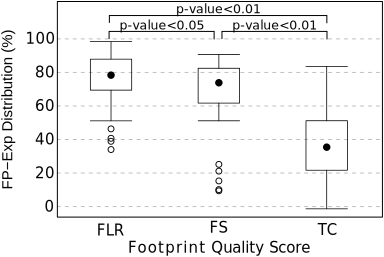
\includegraphics[width=0.5\textwidth]{gusmao_HINT_fpexp_rank}
\caption[Performance of different FP-Exp footprint quality scores]{\textbf{Performance of different FP-Exp footprint quality scores} Distribution of the FP-Exp scores generated using the gene expression evaluation with different footprint quality score metrics. The distributions are based on the values from the three cell type combinations and all the competing methods used.}
\label{fig:gusmao_HINT_fpexp_rank}
\end{figure}

% Table - FN gene exp corrs
\begin{table}[h!]
\footnotesize
\vspace{0.0cm}
\begin{center}
\caption[Friedman-Nemenyi hypothesis test on different FP-Exp footprint quality scores]{\textbf{Friedman-Nemenyi hypothesis test on different FP-Exp footprint quality scores.} Friedman-Nemenyi hypothesis test results on FP-Exp scores generated using the gene expression evaluation with different footprint quality score metrics. The asterisk and the cross, respectively, indicate that the method in the column outperformed the method in the row with significance levels of 0.01 and 0.05.}
\label{tab:fn_gusmao_HINT_chipseq_rank}
\renewcommand{\arraystretch}{1.2}
  \begin{tabular}{ rcc }
    & \rotatebox{90}{FLR} & \rotatebox{90}{FS} \\
    \hline
    FS & $*$ &    \\
    TC & $*$ & $*$   \\
    \hline
  \end{tabular}
\end{center}
\vspace{0.0cm}
\end{table}

%%%%%%%%%%%%%%%%%%%%%%%%%%%%%%%%%%%%%%%%%%%%%%%%%%%%%%%%%%%%%%%%%%%%%
% Section: Impact of DNase-seq Sequence Cleavage Bias
%%%%%%%%%%%%%%%%%%%%%%%%%%%%%%%%%%%%%%%%%%%%%%%%%%%%%%%%%%%%%%%%%%%%%
\subsection{Impact of DNase-seq Sequence Cleavage Bias}
\label{sec:impact.dnase.sequence.cleavage.bias}

% Introduction
In this section we investigate the impact of the DNase-seq sequence cleavage bias on the performance of HINT and whether the correction of such bias improves the footprint prediction accuracy. We tested the two approaches described in Section~\ref{sec:dnase.experimental.bias.correction}: the ``DHS sequence bias'' and the ``naked DNA sequence bias''. The DHS sequence bias considers the sequence bias estimates within DNase hypersensitive sites (DHSs) of each DNase-seq experiment. This approach captures DNase I cleavage bias, read fragmentation and sequence complexity bias of DHSs of each DNase-seq experiment. The naked DNA sequence bias considers the sequence bias estimates within naked DNA DNase-seq experiments. In this case, all DNA regions are open, therefore the sequence bias estimates will mainly capture the DNase I cleavage bias.

% HINT, HINT-BC, HINT-BCN nomenclature
Throughout this section we used the following nomenclature for our computational footprinting method HINT. HINT was evaluated without any DNase-seq sequence bias correction (HINT w/o BC), with the DHS sequence bias correction approach (HINT bias-corrected; HINT-BC) and with the naked DNA sequence bias correction approach (HINT bias-corrected on naked DNase-seq; HINT-BCN).

% TODO below In addition, specially in the DNase-seq bias estimation clustering analysis, we used all cell types from ENCODE's Tier 1 and Tier 2 cell types, generated in Crawford's and Stamatoyannopoulous' labs. See Supplementary Table~\ref{tab:dataencode.dnase} for a full DNase-seq data description and accession numbers.

% Clustering
First, to understand the nature of artifacts on DNase-seq experiments, we analyzed the DNase-seq sequence cleavage bias estimates on all $61$ ENCODE DNase-seq data sets (see Supplementary Table~\ref{tab:dataencode.dnase}). The sequence cleavage bias corresponds to the $6$-mer estimations as shown in Equation~\ref{eq:cleavbias}. These experiments include two existing DNase-seq protocols: the single-hit and double-hit techniques. A clustering analysis of the correlation between the pairwise $6$-mer sequence bias estimates forms two clear groups, which splits experiments from single-hit and double-hit protocols (Figure~\ref{fig:gusmao_bias_cluster_all}). This indicates that sequence biases are protocol-specific. Naked DNA sequence bias estimates forms a sub-cluster within estimates from the double-hit experiments. This highlights that DNase-seq experiments are influenced by more experimental artifacts than DNase sequence cleavage bias alone.

% Figure - Clustering of bias estimates
\begin{figure}[h!]
\centering
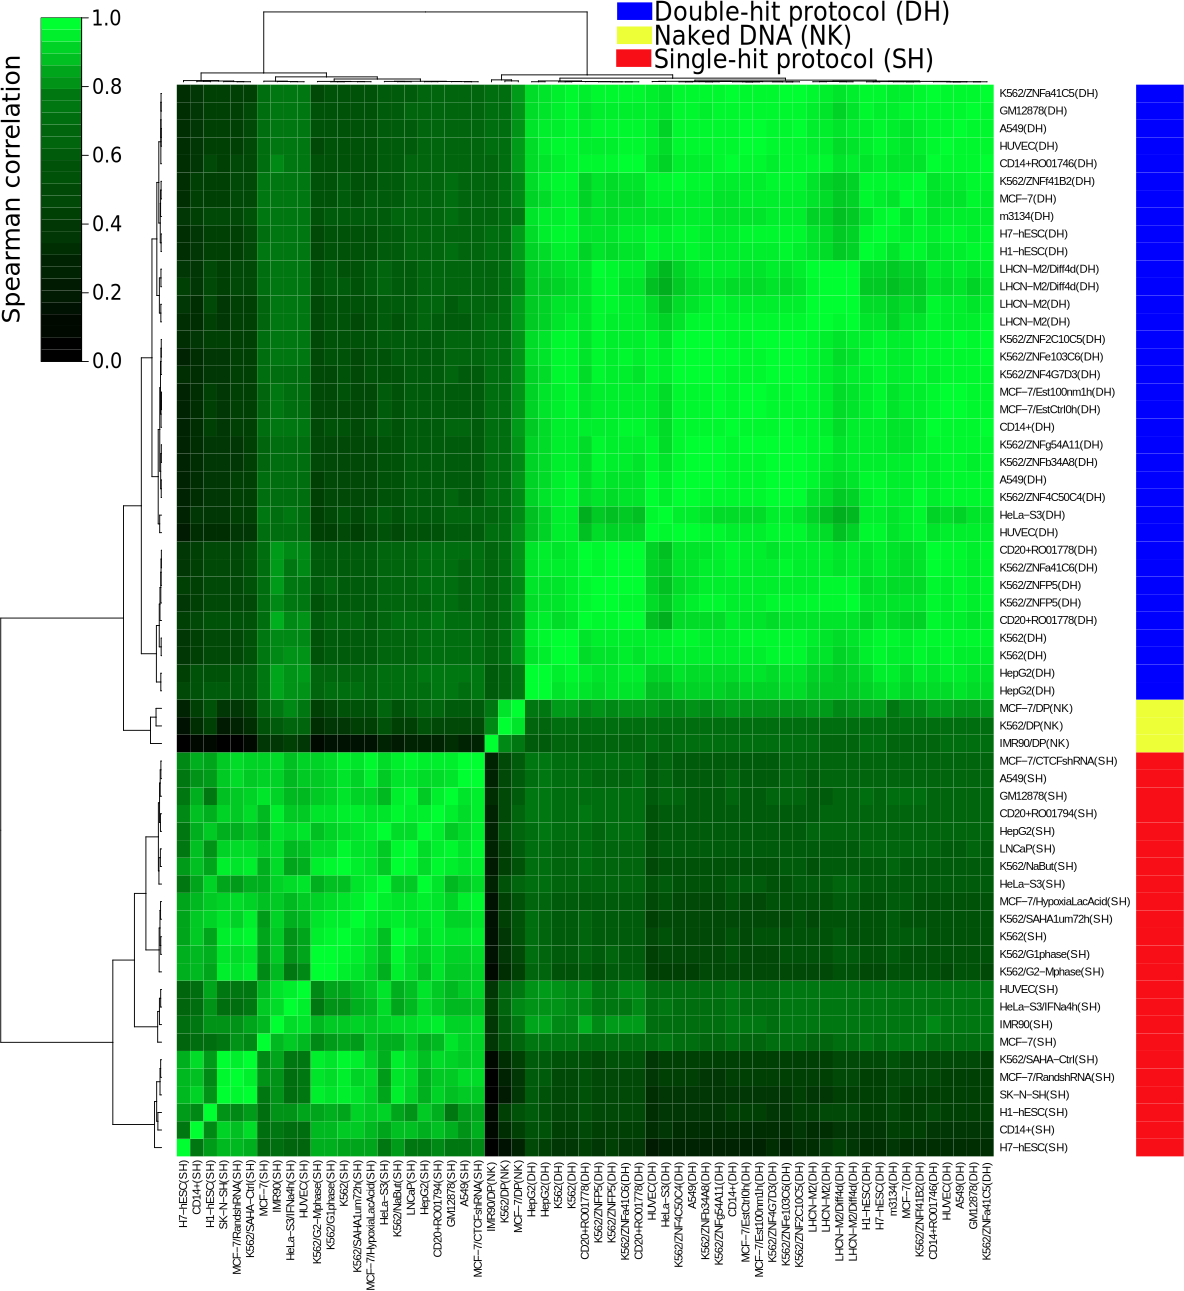
\includegraphics[width=0.99\textwidth]{gusmao_bias_cluster_all}
\caption[Clustering of bias estimates]{\textbf{Clustering of bias estimates.} Ward's minimum variance clustering based on pairwise Spearman correlation coefficient ($r$) from bias estimates (all possible $6$-mers within the DNA alphabet $\{A, C, G, T\}$) of all ENCODE's DNase-seq data and three naked DNA DNase-seq data obtained from different sources. DNase-seq experiments were based on single-hit (red), double-hit (blue) protocols or naked DNA (yellow).}
\label{fig:gusmao_bias_cluster_all}
\end{figure}

% OBS Figure
Next, we extended the analysis by He et al~\cite{he2014} to evaluate the influence of sequence bias on all evaluated footprinting methods. In this analysis we plot, for all computational footprinting methods, the TF-wise amount of bias \emph{vs} the TF-wise footprint prediction accuracy (Figure~\ref{fig:gusmao_bias_obs}a). The amount of bias is calculated as the correlation between the uncorrected DNase-seq signal and the bias signal (Equation~\ref{eq:cleavbias}). Such correlation between observed DNase-seq and predicted bias signal is called ``OBS'' (observed \emph{vs} bias signal). The footprint prediction accuracy is measured through the ChIP-seq evaluation approach using the {\tt Benchmarking Dataset}.

% OBS Results
Our analysis shows that only six out of $14$ evaluated methods (Wellington, Neph, Boyle, DNase2TF, Centipede and FS-Rank) present a significant negative Spearman correlation ($r = -0.35$, $-0.32$, $-0.28$, $-0.28$, $-0.24$ and $-0.22$, respectively) between their accuracy performance and amount of sequence bias (Figure~\ref{fig:gusmao_bias_obs}a; $p$-value $< 0.05$). Equivalent results are also observed on the same TFs and cellular conditions analyzed in He et al.~\cite{he2014}. Methods explicitly using $6$-mer sequence bias statistics (HINT-BC, HINT-BCN and FLR) or performing smoothing (Cuellar, BinDNase and PIQ) are not significantly influenced by sequence bias. Moreover, the performance of HINT-BC is the least affected by sequence bias ($r = -0.06$).

% OBS Results graphs
As an example, we show sequence bias estimates, corrected and uncorrected DNase-seq average profiles around transcription factor binding sites with the highest AUC gain between HINT-BC and HINT w/o BC (Figure~\ref{fig:gusmao_bias_obs}b--c). The NRF1 and EGR1 DNase-seq profiles indicate that the bias-corrected signal fits better their sequence affinity than the uncorrected signal. This means that the higher-affinity parts of NRF1's and EGR1's motif are located in the regions with lowest DNase-seq cleavage.

% Figure - Effects of DNase I sequence cleavage biases on computational footprinting methods
\begin{figure}[h!]
\centering
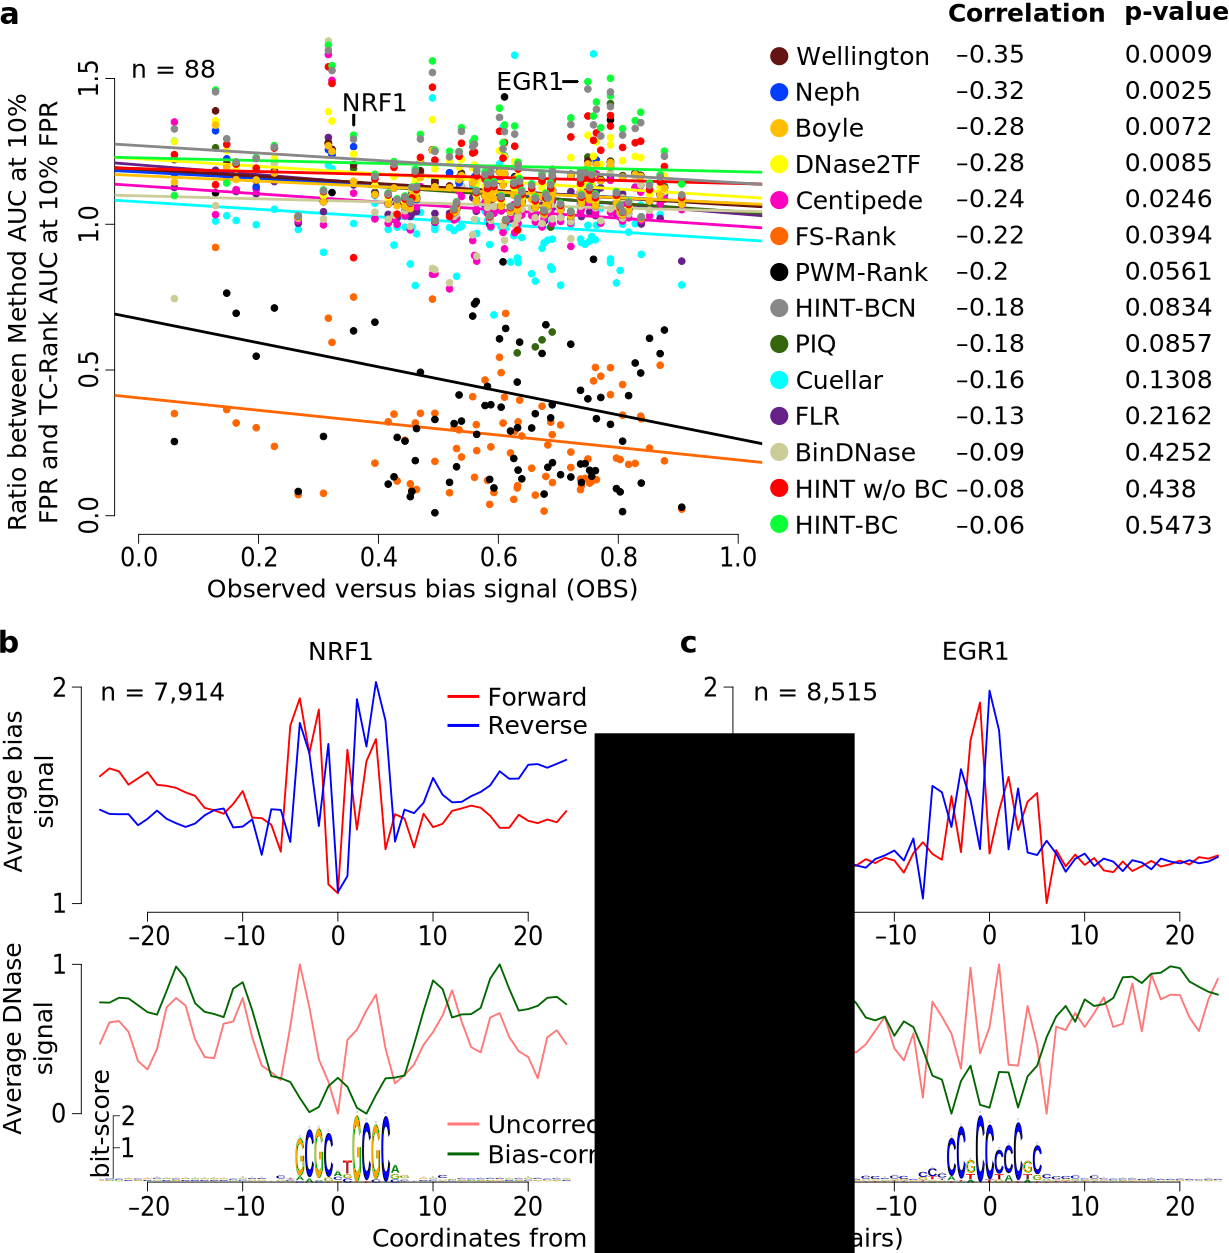
\includegraphics[width=0.99\textwidth]{gusmao_bias_obs}
\caption[Effects of DNase I sequence cleavage biases on computational footprinting methods]{\textbf{Effects of DNase I sequence cleavage biases on computational footprinting methods.} (\textbf{a}) Association between the performance of footprinting methods (relative to TC-Rank performance) and their sequence bias estimated for the transcription factor if the {\tt Benchmarking Dataset}. The $x$-axis represents the correlation between the uncorrected and bias signal (observed \emph{vs} bias signal; OBS). The OBS is evaluated for each TF by measuring the uncorrected DNase-seq signal and the bias signal for every motif-predicted binding site that overlaps a footprint from the evaluated method. Then, the Spearman correlation is evaluated between the average uncorrected and bias signals. Higher OBS values indicate higher bias. The $y$-axis represents the ratio between the AUC at $10\%$ FPR for each evaluated method and the TC-Rank method; higher values indicate higher accuracy. (\textbf{b}--\textbf{c}) Average bias signal (top) and uncorrected/bias-corrected DNase-seq signal (bottom) for the TFs: (\textbf{b}) NRF1 and (\textbf{c}) EGR1. Signals in the bottom graph were standardized to be in the interval $[0,1]$. The motif logo represents all underlying DNA sequences centered on the transcription factor binding sites.}
\label{fig:gusmao_bias_obs}
\end{figure}

% Distribution
Using the same experimental settings as in Figure~\ref{fig:gusmao_bias_obs}, we have investigated more thoroughly the best DNase-seq sequence cleavage bias correction strategy. For that, we evaluated the distribution of the AUC at $10\%$ FPR for HINT w/o BC, HINT-BC and HINT-BCN (Figure~\ref{fig:gusmao_HINT_bias_comparison}). Furthermore, we performed a Friedman-Nemenyi hypothesis test on these three HINT scenarios (Table~\ref{tab:gusmao_HINT_bias_comparison}).

% Comparative results
By analyzing these results, we are able to observe that, although the HINT-BC present slightly higher accuracies than HINT-BCN, these differences are not statistically significant. However, we are able to observe that the accuracies of the HINT-BC strategy significantly outperforms the HINT w/o BC. This is a strong indication that the DNase-seq sequence cleavage bias correction improves the performance of computational footprinting methods. This is an important result since no previous computational footprinting method that used some sort of DNase-seq sequence cleavage bias correction observed significant gain in accuracy~\cite{yardimci2014,sung2014,kahara2015}. Given these results, the DHS sequence cleavage bias correction is the strategy of choice for the application of HINT in all other sections of this chapter.

% Figure - Performance of different bias correction strategies
\begin{figure}[h!]
\centering
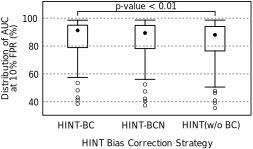
\includegraphics[width=0.6\textwidth]{gusmao_HINT_bias_comparison}
\caption[Performance of different bias correction strategies]{\textbf{Performance of different bias correction strategies.} Distribution of AUC at $10\%$ false positive rate (FPR) of the ROC curves generated using the ChIP-seq evaluation {\tt Comprehensive Dataset} on HINT using: the DHS sequence bias correction (HINT-BC), the naked DNA sequence bias correction (HINT-BCN) and no DNase-seq sequence cleavage bias correction (HINT w/o BC).}
\label{fig:gusmao_HINT_bias_comparison}
\end{figure}

% Table - Friedman-Nemenyi hypothesis test on different bias correction strategies
\begin{table}[h!]
\footnotesize
\vspace{0.0cm}
\begin{center}
\caption[Friedman-Nemenyi hypothesis test on different bias correction strategies]{\textbf{Friedman-Nemenyi hypothesis test on different bias correction strategies.} Friedman-Nemenyi hypothesis test results on AUC at $10\%$ false positive rate (FPR) of the ROC curves generated using the ChIP-seq evaluation {\tt Benchmarking Dataset} on different bias correction strategies. The asterisk and the cross, respectively, indicate that the method in the column outperformed the method in the row with significance levels of 0.01 and 0.05.}
\label{tab:gusmao_HINT_bias_comparison}
\renewcommand{\arraystretch}{1.2}
  \begin{tabular}{ rccc }
    & \rotatebox{90}{HINT-BC} & \rotatebox{90}{HINT-BCN}  \\
    \hline
    HINT-BCN &  &    \\
    HINT(w/o BC) & $*$ &   \\
    \hline
  \end{tabular}
\end{center}
\vspace{0.0cm}
\end{table}

% CG content intro
Nevertheless, claims have been made with regard to the DNase-seq sequence cleavage bias correction and the fact that many transcription factors present CG-rich motifs~\cite{sung2014}. Since the transcription factors have a sequence binding affinity preference, which in many cases is composed of C and G nucleotides, the DNase-seq sequence cleavage bias correction could be simply creating ``artifact'' peak-dip-peak patterns on the DNase-seq data, since the DNase I enzyme also has a preference to bind CG-rich motifs.

% CG content results
To investigate such claim we evaluated the distribution of the pairwise AUC differences between the three HINT versions (HINT w/o BC, HINT-BC and HINT-BCN) for all transcription factors of the {\tt Comprehensive Dataset} gold standard (Figure\ref{fig:gusmao_bias_cg}a). Furthermore, we also evaluated the CG content of these transcription factor motifs (Figure~\ref{fig:gusmao_bias_cg}b). 

% CG content results
By analyzing the Figure~\ref{fig:gusmao_bias_cg}a--b we observe no correlation between CG content of the motifs and the individual AUC of each method: HINT (w/o BC) $ r = -0.0144$, HINT-BC $ r = 0.0254$ and HINT-BCN $ r = 0.0108$ ($p$-value $> 0.05$; Spearman correlation test). Furthermore, we observe no correlation between CG content of motifs and differences in AUC: HINT-BC $-$ HINT-BCN $ r = 0.0188$, HINT-BC $-$ HINT (w/o BC) $ r = 0.0724$ and HINT-BCN $-$ HINT (w/o BC) $ r = 0.0644$ ($p$-value $> 0.05$; Spearman correlation test). This is evidence that the DNase-seq sequence cleavage bias is not due to artifacts generated by protein-DNA interaction preferences of both the DNase I enzyme and the transcription factors.

% Figure - Evaluation of bias correction strategies and CG content contribution
\begin{figure}[h!]
\centering
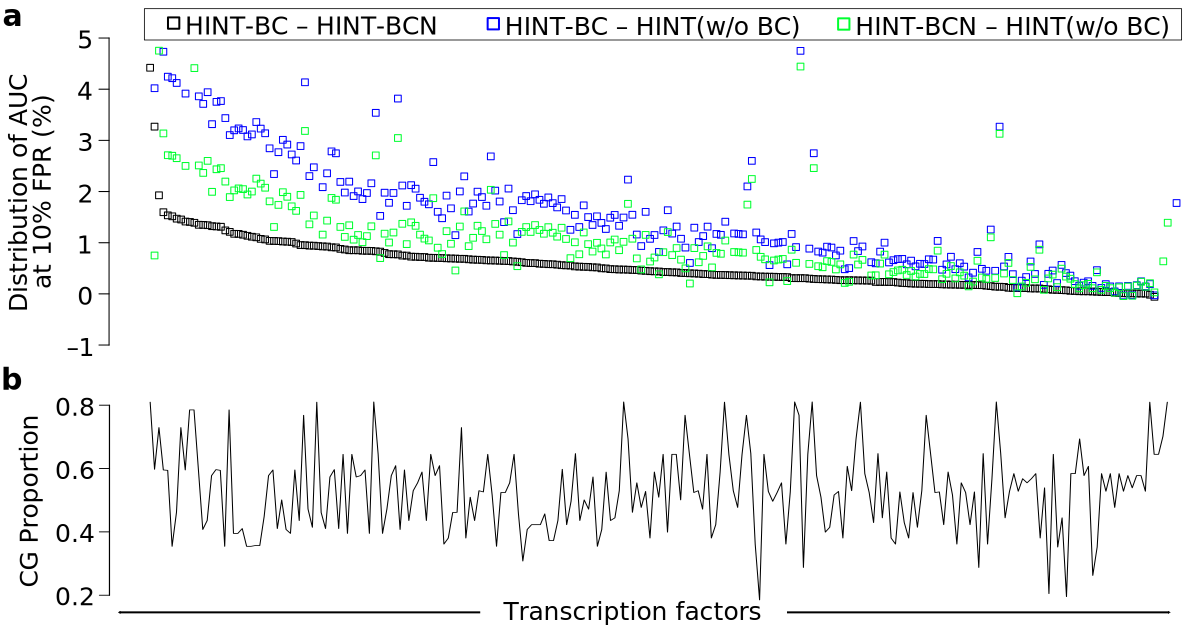
\includegraphics[width=0.8\textwidth]{gusmao_bias_cg}
\caption[Evaluation of bias correction strategies and CG content contribution]{\textbf{Evaluation of bias correction strategies and CG content contribution.} (\textbf{a}) Distribution of AUC ($10\%$ FPR) differences bettween HINT-BC and HINT (w/o BC), HINT-BCN and HINT (w/o BC); HINT-BC and HINT-BCN for the {\tt Comprehensive Dataset}. Transcription factors are ranked by the difference between HINT-BC and HINT-BCN. (\textbf{b}) CG content of transcription factors. The CG content is calculated as $\frac{n_C+n_G}{n_A+n_C+n_G+n_T}$, where $n_X$ is the frequency of the nucleotide $X$ in all transcription factor binding sites.}
\label{fig:gusmao_bias_cg}
\end{figure}

% Contingency table test
Finally, to understand the computational mechanism in which the DNase-seq sequence cleavage bias correction improves the accuracy of HINT, we generated DNase-seq profiles with uncorrected and bias-corrected signals in transcription factor binding sites that matched true positive (TP), false negative (FN), false positive (FP) and true negative (TN) predictions (i.e. the contingency table from the ChIP-seq evaluation scheme). The results of such analysis is presented in Figure~\ref{fig:gusmao_bias_contingency_profile} for three selected transcription factors: GABP, NRF1 and EGR1. This figure shows, for all transcription factors and signal types, the clear peak-dip-peak DNase-seq profile (i.e. the grammar of active transcription factor binding sites) for the true positive predictions and a complete lack of such average pattern for the true negatives.

% Contingency table results
The profile around the false positive predictions are virtually the same between the uncorrected and bias-corrected DNase-seq signals. However, we are able to observe that the profiles around false negative predictions are significantly lower in intensity and different in shape ($p$-value $< 0.01$; Mann-Whitney-Wilcoxon on the DNase-seq signal distribution at flanking regions and motif center) regarding the bias-corrected signal, in comparison to the uncorrected case. This shows that the DNase-seq sequence cleavage bias correction strategy enhances the accuracy by correctly predicting transcription factors that would not be otherwise predicted without such correction. Such observation is in line with the fact that we observe a clearer dip-peak-dip pattern in the average DNase-seq signal for multiple transcription factors (see Figure~\ref{fig:gusmao_bias_obs}b--c).

% Figure - Uncorrected and bias-corrected DNase-seq profile between different contigency table statistics
\begin{figure}[h!]
\centering
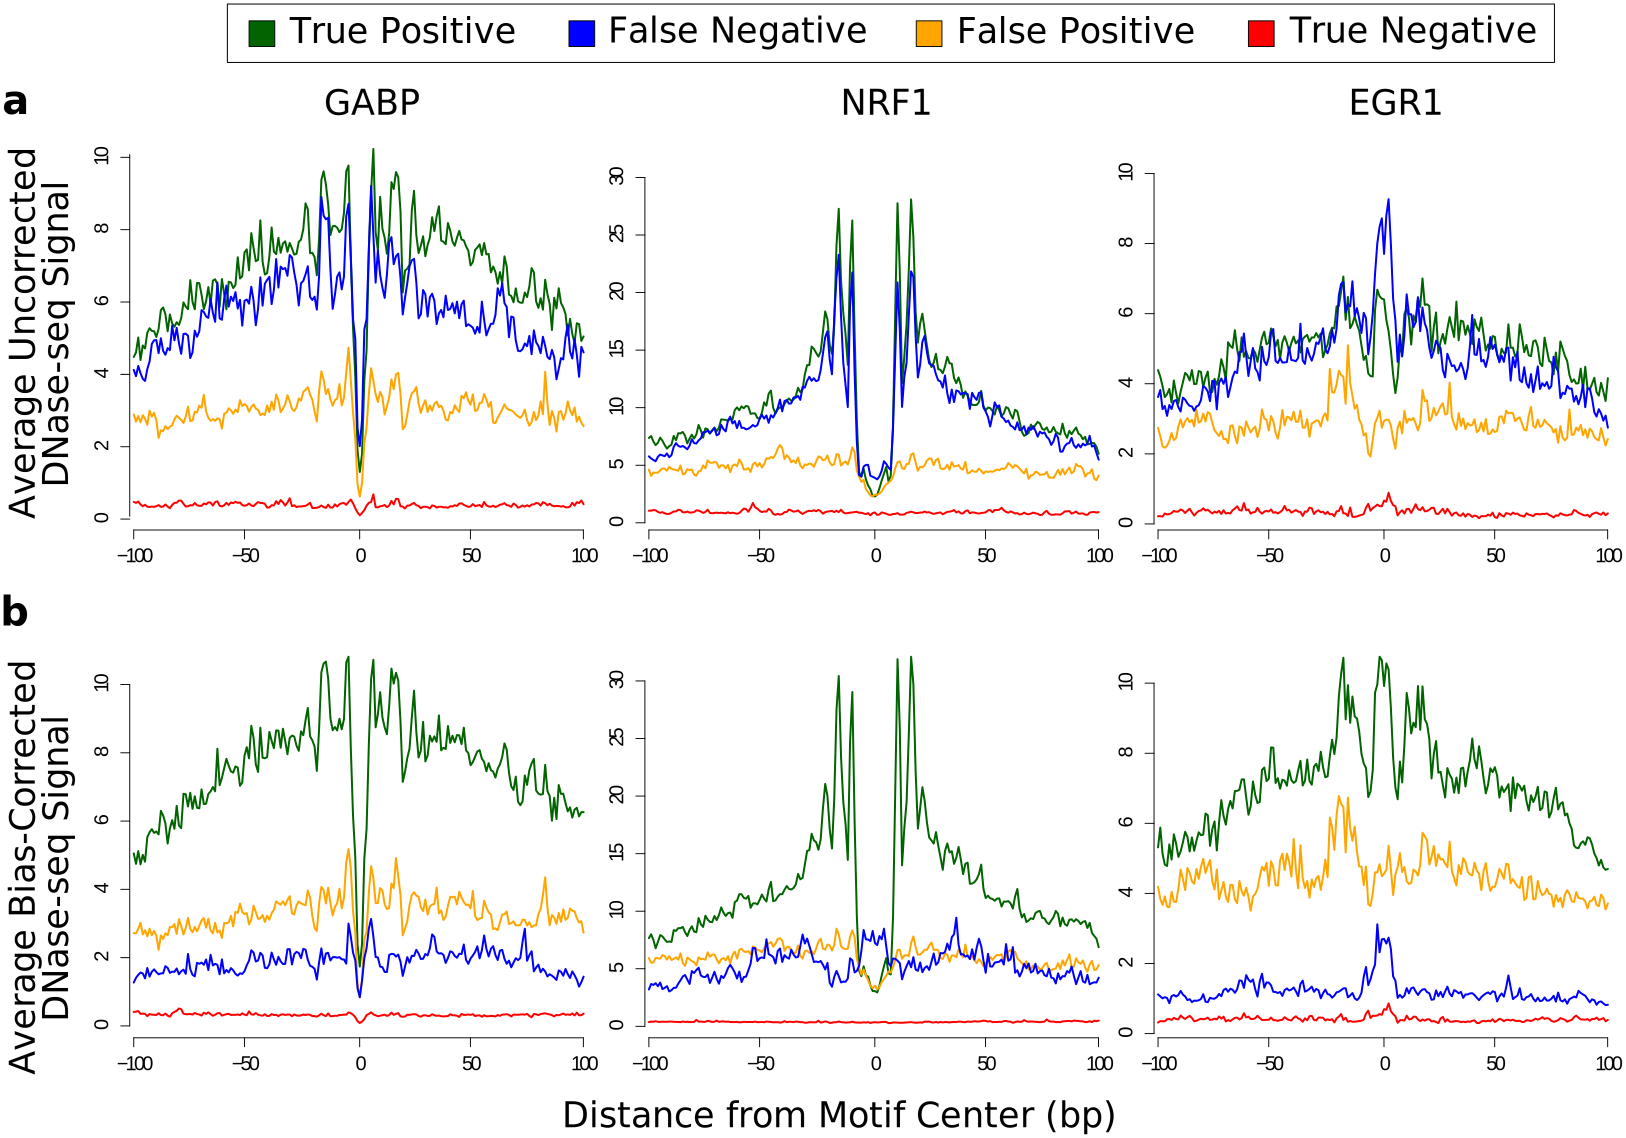
\includegraphics[width=0.99\textwidth]{gusmao_bias_contingency_profile}
\caption[Uncorrected and bias-corrected DNase-seq profile between different contigency table statistics]{\textbf{Uncorrected and bias-corrected DNase-seq profile between different contigency table statistics.} This figure shows the uncorrected (top graphs) and bias-corrected (bottom graphs) DNase-seq signal centered at HINT's true positive (TP), false negative (FN), false positive (FP) and true negative (TN) predictions of the binding site of trascription factors GABP, NRF1 and EGR1.}
\label{fig:gusmao_bias_contingency_profile}
\end{figure}

% Conclusion / de novo motifs
An example that ignoring experimental artifacts might lead to false predictions can be seen in Figure~\ref{fig:gusmao_neph_denovo_bias}. In this figure we show the DNase-seq profile for two motifs (termed 0458 and 0500) found on Neph footprint predictions which did not match any existing known motif (i.e. \emph{de novo} transcription factor motifs). Bias corrected DNase-seq profiles reveal very weak footprint shape. Furthermore, we compared the overlap between footprints generated by HINT-BC and Neph in the same cell type in which these \emph{de novo} motifs were found (H7-hESC). We observed that $24.99\%$ (motif 0458) and $28.58\%$ (motif 0500) of motif-predicted binding sites associated with a Neph footprint. In contrast, only $0.73\%$ (motif 0458) and $1.71\%$ (motif 0500) of motif-predicted binding sites overlapped with a HINT-BC footprint. Altogether, this indicates that these motifs are indeed potential artifacts of cleavage bias and reinforces the importance of bias correction prior to any DNase-seq analysis.

% Figure - Average bias and DNase-seq signals around binding sites of Neph's \emph{de novo} motifs
\begin{figure}[h!]
\centering
\includegraphics[width=0.99\textwidth]{gusmao_neph_denovo_bias}
\caption[Average bias and DNase-seq signals around binding sites of Neph's \emph{de novo} motifs]{\textbf{Average bias and DNase-seq signals around binding sites of Neph's \emph{de novo} motifs.} Average bias and DNase-seq signals around binding sites of \emph{de novo} motifs 0458 and 0500 on cell type H7-hESC. In the top panel, we show the strand-specific average DNase-seq signal on naked DNA DNase-seq experiments (MCF-7 cell type); the middle panel shows the strand-specific estimated cleavage bias signal; and the bottom panels shows the (1) uncorrected -- observed DNase-seq I cleavage signal and (2) corrected -- DNase-seq signal after the bias correction by using Equation~\ref{eq:cleavbias}. Bottom panel signals were standardized to be in $[0,1]$. Below the graphs, it is shown the motif logo estimated on the DNA sequences of these regions. These motifs were discovered in the footprint analysis of~\cite{neph2012a} and indicated in~\cite{he2014} to be possible artifacts of cleavage bias.}
\label{fig:gusmao_neph_denovo_bias}
\end{figure}





























%%%%%%%%%%%%%%%%%%%%%%%%%%%%%%%%%%%%%%%%%%%%%%%%%%%%%%%%%%%%%%%%%%%%%
% Section: Computational Footprinting Methods Comparison
%%%%%%%%%%%%%%%%%%%%%%%%%%%%%%%%%%%%%%%%%%%%%%%%%%%%%%%%%%%%%%%%%%%%%
\section{Computational Footprinting Methods Comparison}
\label{sec:computational.footprinting.methods.comparison}

% Introduction / Methods
In this section we present a comprehensive comparative analysis of HINT and all competing computational footprinting methods. Since most competing methods use only DNase-seq data, we used the DNase-only HINT topology for a fairer comparison. HINT's DNase-seq cleavage bias correction strategy followed the DHS cleavage bias scheme. Both HINT and competing methods were executed exactly as described in Chapter~\ref{cha:experiments}.

% Introduction subsections
The computational footprinting method comparison was performed using: (1) the ChIP-seq evaluation method with the {\tt Benchmarking Dataset} (Section~\ref{sec:mc.chipseq.evaluation}) and (2) the gene expression evaluation method (Section~\ref{sec:mc.gene.expression.evaluation}). We close this section with a discussion on both evaluation methodologies in an integrated comparison showing the full experimental result's picture (Section~\ref{sec:integrated.comparison}).

%%%%%%%%%%%%%%%%%%%%%%%%%%%%%%%%%%%%%%%%%%%%%%%%%%%%%%%%%%%%%%%%%%%%%
% Section: ChIP-seq Evaluation
%%%%%%%%%%%%%%%%%%%%%%%%%%%%%%%%%%%%%%%%%%%%%%%%%%%%%%%%%%%%%%%%%%%%%
\subsection{ChIP-seq Evaluation}
\label{sec:mc.chipseq.evaluation}

% Intro - ROC / PR
In the ChIP-seq evaluation approach, we create ROC and PR curves for each method on the prediction of each transcription factor in our {\tt Benchmark Dataset}. The Figure~\ref{fig:gusmao_roc_pr} shows examples of ROC and PR curves for the transcription factors EGR1, GABP and C-JUN. At first glance we are able to observe that the site-centric baseline methods FP-Rank and PWM-Rank present the lowest accuracies. Furthermore, the site-centric baseline method TC-Rank and the segmentation baseline method Filter exhibit a good performance. The Filter method often outperformed more complex computational footprinting methods (Cuellar, FLR and Centipede). The higher-ranked computational footprinting methods (HINT, DNase2TF and PIQ) have very close AUC at $100\%$ FPR. However, the PR curves in Figure~\ref{fig:gusmao_roc_pr} show us that these methods compete with regard to the delay in sensitivity decrease as specificity increases. This is the main reason in which we also evaluated the AUC at lower FPR levels and the AUPR.

% Figure - Example of ROC and PR curves
\begin{figure}[h!]
\centering
\includegraphics[width=0.99\textwidth]{gusmao_roc_pr}
\caption[Example of ROC and PR curves]{\textbf{Example of ROC and PR curves.} (\textbf{a}) Example of ROC curves for the transcription factors EGR1, GABP, and C-JUN. Each graph depicts a curve of a different color for each of the $14$ computational footprinting methods evaluated. The legend on each graph shows the AUC at $100\%$ FPR. (\textbf{b}) Example of PR curves for the transcription factors EGR1, GABP, and C-JUN. The legend on each graph shows the AUPR for all $14$ evaluated methods.}
\label{fig:gusmao_roc_pr}
\end{figure}

% Boxplot
To have a better perspective of the results for all methods and transcription factors tested we evaluated the distribution of the AUC at $100\%$, $10\%$ and $1\%$ FPR as well as the AUPR (Figure~\ref{fig:gusmao_chipseq_method_comparison}). AUC at lower FPRs favors methods with higher sensitivity in expense of specificity. Also, AUC at lower FPRs tend to get closer results to the AUPR, which is ideal for very imbalanced classification problems. We observe the importance of using cell-specific open chromatin data (in this case, DNase-seq) by analyzing the dramatic increase in accuracy from the PWM method to all other methods that use such open chromatin data. The only exception to this remark is the FS-Rank method, which uses DNase-seq data but does present lower average accuracies than the PWM method. However, note that the FS metric, when combined with footprint predictions, generally present higher accuracies than the PWM metric (see Section~\ref{sec:frs.chipseq.evaluation}). The reason for such lower FS-Rank accuracies stems from its inability to model the length of the DNase-seq depletion and peaks given that the FS-Rank relies on a fixed-window length strategy.

% Comparison
The Figure~\ref{fig:gusmao_chipseq_method_comparison} shows that the HINT method is the best method with regard to all metrics tested. HINT is closely followed by DNase2TF, PIQ and Wellington. It is interesting to observe that all segmentation methods are in the top-six positions of the rank for all metrics. This suggests that segmentation methods outperform site-centric approaches on the detection of active binding sites. Moreover, the results from the different evaluation statistics result in very similar rankings ($r > 0.98$).

% Figure - ChIP-seq evaluation accuracy distributions
\begin{figure}[h!]
\centering
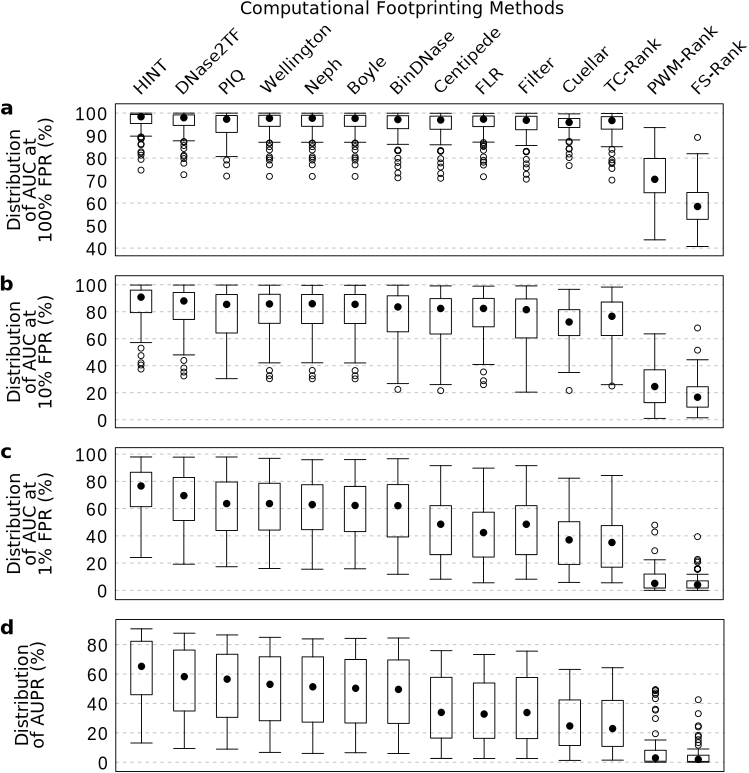
\includegraphics[width=0.99\textwidth]{gusmao_chipseq_method_comparison}
\caption[ChIP-seq evaluation accuracy distributions]{\textbf{ChIP-seq evaluation accuracy distributions.} Accuracy distribution for $14$ footprinting methods regarding all validation sets (ordered by Friedman Ranking). The accuracy is given by the statistics: (\textbf{a}) AUC at $100\%$ FPR (\textbf{b}) AUC at $10\%$ FPR (\textbf{c}) AUC at $1\%$ FPR and (\textbf{d}) AUPR.}
\label{fig:gusmao_chipseq_method_comparison}
\end{figure}

%%%%%%%%%%%%%%%%%%%%%%%%%%%%%%%%%%%%%%%%%%%%%%%%%%%%%%%%%%%%%%%%%%%%%
% Section: Gene Expression Evaluation
%%%%%%%%%%%%%%%%%%%%%%%%%%%%%%%%%%%%%%%%%%%%%%%%%%%%%%%%%%%%%%%%%%%%%
\subsection{Gene Expression Evaluation}
\label{sec:mc.gene.expression.evaluation}

% Introduction
In the gene expression evaluation we evaluate the correlation between changes in gene expression for a number of transcription factors with differences in the quality of footprint predictions for these factors. To measure the change in gene expression we use the gene expression fold change (FC). The quality metric of footprints used is the footprint likelihood ratio (FLR). Differences in such footprint quality metric is measures with the Kolmogorov-Smirnov (KS) test statistic. The Spearman correlation between FLR score difference and expression FC, which we refer to as FP-Exp, will be used to rank footprinting methods. Higher FP-Exp values indicate better performance. The gene expression evaluation methodology only requires expression data and is therefore more generally applicable than the ChIP-seq evaluation. However, differently from the ChIP-seq evaluation, the gene expression approach cannot evaluate footprint predictions of individual transcription factors.

% General results
We observed high average FP-Exp values for the majority of evaluated methods (FP-Exp $ = 0.79$) and extremely high FP-Exp values (FP-Exp $ > 0.9$) for top performing methods on comparisons between pairs of cell types H1-hESC, K562 and GM12878 (Figure~\ref{fig:gusmao_fpexp_method_comparison}). Moreover, similar rankings of methods are obtained for each cell pair: H1-hESC/K562 \textit{vs} H1-hESC/GM12878 $r = 0.99$, H1-hESC/K562 \textit{vs} GM12878/K562 $r = 0.96$, and H1-hESC/GM12878 \textit{vs} GM12878/K562 $r = 0.97$. We also observed a high agreement between the ranking of computational footprinting methods using the gene expression evaluation methodology and the ranking of methods using the ChIP-seq evaluation approach ($r > 0.88$).

% Method-wise results
In Figure~\ref{fig:gusmao_fpexp_method_comparison} we show the top four methods with regard to the gene expression evaluation. Since a single FP-Exp is evaluated for a collection of transcription factors, it is not possible to graphically display the distribution of accuracies as in the ChIP-seq evaluation scheme. Nevertheless, we are able to observe that HINT is again the top-ranked method, followed by DNase2TF, Neph and FLR.

% Figure - Correlation between KS statistic and FC expression for different cell pairs
\begin{figure}[h!]
\centering

\includegraphics[width=0.99\textwidth]{gusmao_fpexp_method_comparison}
\caption[Gene expression evaluation accuracy correlations (FP-Exp)]{\textbf{Gene expression evaluation accuracy correlations (FP-Exp).} Correlation between KS statistics from FLR scores \textit{vs} fold change expression for cell type pairs H1-hESC \textit{vs} K562 (left), H1-hESC \textit{vs} GM12878 (middle) and GM12878 \textit{vs} K562 (right) for footprints predicted by: HINT, DNase2TF, Neph and FLR (from top to bottom, respectively). }
\label{fig:gusmao_fpexp_method_comparison}
\end{figure}

%%%%%%%%%%%%%%%%%%%%%%%%%%%%%%%%%%%%%%%%%%%%%%%%%%%%%%%%%%%%%%%%%%%%%
% Section: Integrated Comparison
%%%%%%%%%%%%%%%%%%%%%%%%%%%%%%%%%%%%%%%%%%%%%%%%%%%%%%%%%%%%%%%%%%%%%
\subsection{Integrated Comparison}
\label{sec:integrated.comparison}

% Figure and FN
We integrated all the computational footprinting method's results to perform a global comparison. The Figure~\ref{fig:gusmao_method_comparison} shows the ranking of all computational footprinting methods with regard to all evaluation metrics: FP-Exp, AUCs (at $100\%$, $10\%$ and $1\%$ FPR) and AUPR. Furthermore, we combined all these results and performed a Friedman-Nemenyi test for statistical significance (Table~\ref{tab:fn.table.aupr}).

% Results
HINT has the highest FP-Exp, AUC and AUPR values and significantly outperforms all methods ($p$-value $< 0.01$). The next top performing method is DNase2TF, which significantly outperforms all other methods except PIQ ($p$-value $< 0.05$ for Wellington; $p$-value $< 0.01$ for all others). PIQ outperforms all of its lower ranked competitors but Wellington ($p$-value $< 0.05$ for Neph; $p$-value $< 0.01$ for all others).

% Segmentation vs site-centric
The segmentation methods HINT, DNase2TF, Wellington and Neph are ranked within the top five methods regarding all evaluation metrics, individually. Boyle is the only segmentation method not included within the top five; however it displayed good accuracies (placed $6^{\text{th}}$ in the global ranking). The site-centric method PIQ obtained the best accuracies among the site-centric methods (placed $3^{\text{rd}}$ in the global ranking). All site-centric baseline methods (FS-Rank, PWM-Rank and TC-Rank) are in the bottom four positions of the ranks. These results lead us to claim that the segmentation approach is preferable over the site-centric approach.

% Figure - Evaluation of computational footprinting methods
\begin{figure}[h!]
\centering
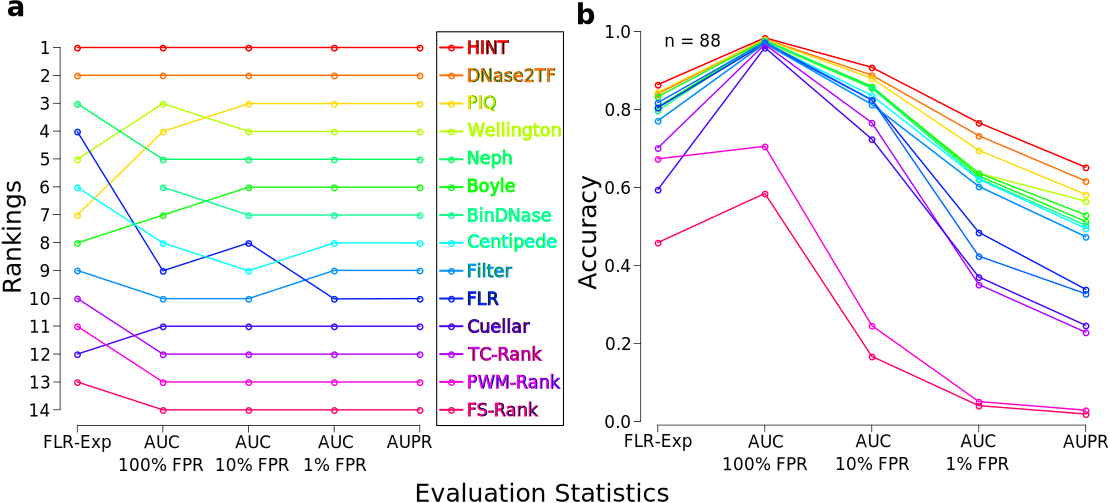
\includegraphics[width=0.99\textwidth]{gusmao_method_comparison}
\caption[Evaluation of computational footprinting methods]{\textbf{Evaluation of computational footprinting methods.} (\textbf{a}) Average rankings for the evaluated computational footprinting methods. The rankings are given for all evaluation criteria: FP-Exp, ChIP-seq evaluation AUC (at $100\%$, $10\%$ and $1\%$ FPR) and AUPR. (\textbf{b}) For all evaluated methods we show the FP-Exp values (as a combination of all pairwise comparison within cell types H1-hESC, K562 and GM12878), median ChIP-seq evaluation AUC (at $100\%$, $10\%$ and $1\%$ FPR) values and median AUPR values. Note that BinDNase could not be evaluated with the gene expression approach, as it requires transcription factor ChIP-seq data for training.}
\label{fig:gusmao_method_comparison}
\end{figure}

% Table - Friedman-Nemenyi hypothesis test on different computational footprinting methods
\begin{table}[h!]
\footnotesize
\vspace{0.0cm}
\begin{center}
\caption[Friedman-Nemenyi hypothesis test on different computational footprinting methods]{\textbf{Friedman-Nemenyi hypothesis test on different computational footprinting methods.} Friedman-Nemenyi hypothesis test results for all computational footprinting methods evaluated on the distribution of all tested metrics: FP-Exp, AUCs and AUPR. The asterisk and the cross, respectively, indicate that the method in the column outperformed the method in the row with significance levels of 0.01 and 0.05.}
\label{tab:fn.table.aupr}
\renewcommand{\arraystretch}{1.2}
  \begin{tabular}{ rcccccccccccccc }
    & \rotatebox{90}{HINT} & \rotatebox{90}{DNase2TF} & \rotatebox{90}{PIQ} & \rotatebox{90}{Wellington} & \rotatebox{90}{Neph} & \rotatebox{90}{Boyle} & \rotatebox{90}{BinDNase} & \rotatebox{90}{FLR} & \rotatebox{90}{Centipede} & \rotatebox{90}{Filter} & \rotatebox{90}{Cuellar} & \rotatebox{90}{TC} & \rotatebox{90}{PWM} \\
    \hline
    DNase2TF & $*$ &     &     &     &     &     &     &     &   &   &     &     &          \\
    PIQ & $*$ &     &     &     &     &     &     &     &     &  &   &     &          \\
    Wellington & $*$ & $+$ &     &     &     &     &     &     &  &   &     &     &          \\
    Neph & $*$ & $*$ & $+$ &     &     &     &     &     &     &  &   &     &          \\
    Boyle & $*$ & $*$ & $*$ &     &     &     &     &     &     &  &   &     &          \\
    BinDNase & $*$ & $*$ & $*$ &     &     &     &     &     &  &   &     &     &          \\
    FLR & $*$ & $*$ & $*$ & $*$ & $*$ & $*$ & $*$ &     &     &  &   &     &          \\
    Centipede & $*$ & $*$ & $*$ & $*$ & $*$ & $+$ & $+$ &     &  &   &     &     &          \\
    Filter & $*$ & $*$ & $*$ & $*$ & $*$ & $*$ & $*$ & $*$ &   &  &     &     &          \\
    Cuellar & $*$ & $*$ & $*$ & $*$ & $*$ & $*$ & $*$ & $*$ &   &  &     &     &          \\
    TC & $*$ & $*$ & $*$ & $*$ & $*$ & $*$ & $*$ & $*$ & $+$  &    &     &     &          \\
    PWM & $*$ & $*$ & $*$ & $*$ & $*$ & $*$ & $*$ & $*$ & $*$ & $*$ &     &     &          \\
    FS & $*$ & $*$ & $*$ & $*$ & $*$ & $*$ & $*$ & $*$ & $*$ & $*$ & $+$ &     &          \\
    \hline
  \end{tabular}
\end{center}
\vspace{0.0cm}
\end{table}























%%%%%%%%%%%%%%%%%%%%%%%%%%%%%%%%%%%%%%%%%%%%%%%%%%%%%%%%%%%%%%%%%%%%%
% Section: De Novo Motif Finding on Predicted Footprints
%%%%%%%%%%%%%%%%%%%%%%%%%%%%%%%%%%%%%%%%%%%%%%%%%%%%%%%%%%%%%%%%%%%%%
\section{\emph{De Novo} Motif Finding on Predicted Footprints}
\label{sec:denovo.motif.finding.footprints}

% Introduction
The predicted footprints from a segmentation computational footprinting approach represent a map of active transcription factor binding sites. In possession of such regulatory landscape one might be able to perform many downstream analysis. Here we present an example of such analysis -- the \emph{de novo} motif finding. This analysis consists on searching for novel transcription factor DNA affinity sequences which do not match any known affinity sequence in the literature.

% Method
We performed a \emph{de novo} motif finding analysis on footprints predicted by HINT on cell type H1-hESC. First, we applied a massive motif matching on all $738,707$ predicted footprints using all PFMs from the Jaspar and Uniprobe repositories. Before the motif matching, we extended all footprints by $10$ bp to each side to be able to recognize larger sequence motifs. We observed that \approxy$5.37\%$ ($39,703$) of H1-hESC's footprints did not present any motif-predicted binding site. Then, we applied the \emph{de novo} motif finding tool DREME (discriminative regular expression motif elicitation)~\cite{bailey2011} on these footprints that did not present any known motif. Such tool is optimized to perform \emph{de novo} motif analysis in datasets containing many sequences and is able to find multiple different motifs. Briefly, DREME finds substrings that appear in a target genomic region set (in our case, the footprints) more frequent than by chance given a background genomic region set (in our case, random genomic regions with the same length of the footprints but with $100$ times more sequences). In addition, we also executed the CENTRIMO (local motif enrichment analysis)~\cite{bailey2012} tool on all sequences associated to the \emph{de novo} motifs found by DREME. This tool makes sure that the motifs found are centrally enriched within the footprints and are not a product of the $10$ bp extension we performed.

% Results
Given the quality scores given by DREME and CENTRIMO, we were able to find six very frequent motifs in H1-hESC which did not match with any existing motif from the repositories used. The Figure~\ref{fig:gusmao_denovo} shows these six motifs and their DREME $p$-value. Each motif is named after its IUPAC consensus sequence standards. We also show in Figure~\ref{fig:gusmao_denovo} the average DNase-seq signal on a $200$ bp window around each of these \emph{de novo} motifs (DNase-seq profile graph). We are able to see that, with exception of the TACCCR motif, all other motifs presented a very clear peak-dip-peak DNase-seq pattern, consistent with the grammar of active transcription factor binding sites. Furthermore, we are able to see that the motifs CKCSGAG and CCGGAGHC present very clear signs of co-binding. This can be seen as a pattern of multiple dips with a $10$--$15$ bp spacing between them, instead of a single dip in the middle of the DNase-seq profile graphs.

% Figure - de novo TF motifs predicted on H1-hESC with HINT's footprints
\begin{figure}[h!]
\centering
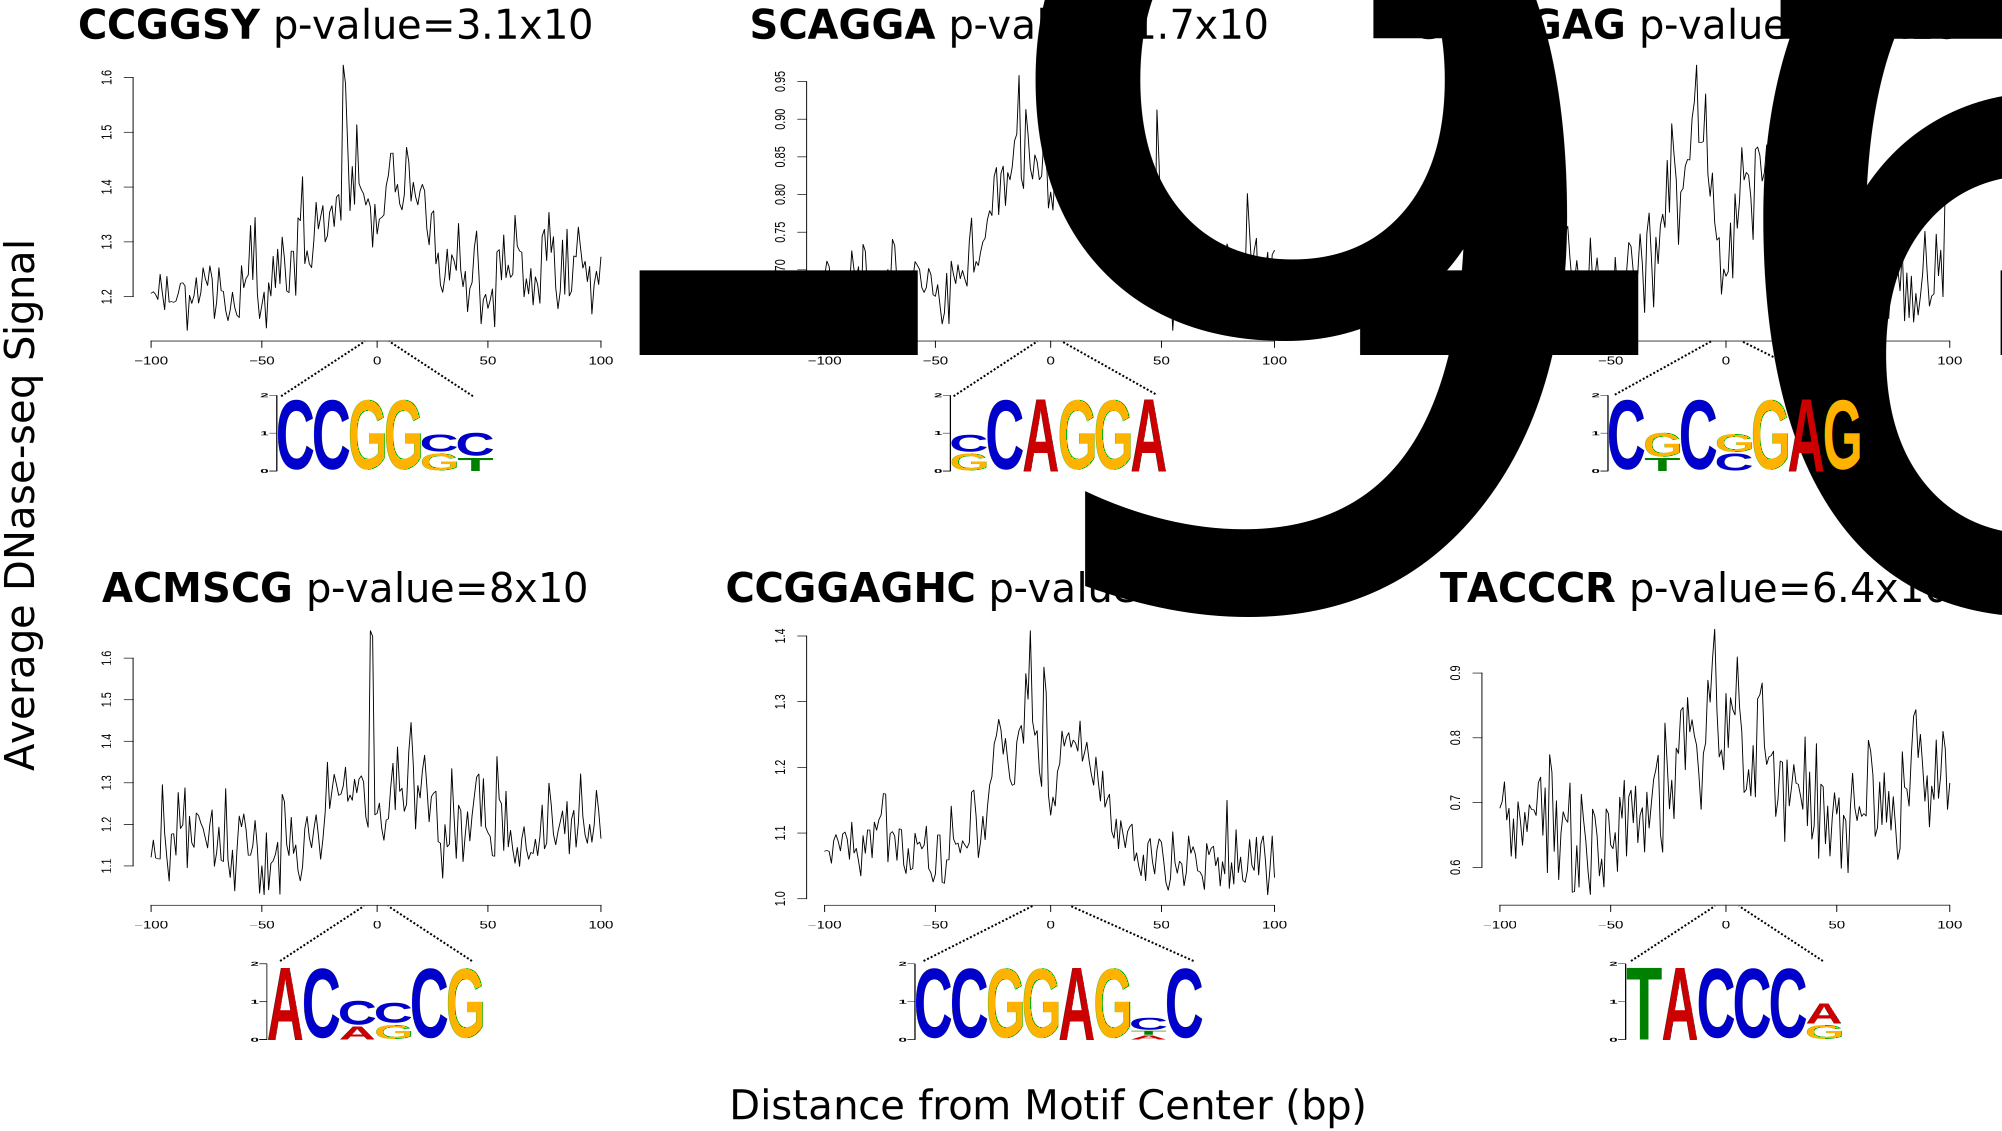
\includegraphics[width=0.99\textwidth]{gusmao_denovo}
\caption[\emph{De novo} TF motifs predicted on H1-hESC with HINT's footprints]{\textbf{\emph{De novo} TF motifs predicted on H1-hESC with HINT's footprints.} We show six \emph{de novo} motifs which satisfied all quality checks after the application of DREME and CENTRIMO softwares on H1-hESC's HINT footprint predictions which did not match any known DNA sequence affinity motif. Each motif is named after its IUPAC consensus sequence (bold, top of each graph) and the $p$-value of the DREME analysis is also shown. The graphs represent the average DNase-seq signal around a $200$ bp window centered on motif-predicted binding sites found in the whole genome after applying each \emph{de novo} PFM. The motif sequence logo is shown below each \emph{de novo} motif's graph.}
\label{fig:gusmao_denovo}
\end{figure}

% Conclusion
Needless to say, such \emph{de novo} motifs need to be experimentally validated using biological methods. However, the fact that we are able to see a peak-dip-peak pattern on the DNase-seq profile is a very high indicative of active transcription factor binding. The intent of this analysis was to show an example of downstream post hoc analysis using footprints predicted with HINT. In Section~\ref{sec:case.studies} we will show the application of footprints on real biological scenarios in which positive inferences could be performed.

























%%%%%%%%%%%%%%%%%%%%%%%%%%%%%%%%%%%%%%%%%%%%%%%%%%%%%%%%%%%%%%%%%%%%%
% Section: Impact of Transcription Factor Residence Time
%%%%%%%%%%%%%%%%%%%%%%%%%%%%%%%%%%%%%%%%%%%%%%%%%%%%%%%%%%%%%%%%%%%%%
\section{Impact of Transcription Factor Residence Time}
\label{sec:impact.tf.residence.time}

% TODO - Falar onde obteve os de novo do Neph
% \emph{De novo} PFMs 0458 and 0500 were downloaded from Neph et al.~\cite{neph2012a}.

% Introduction - nuclear receptors
Despite the high average prediction values of top performing footprint methods, they consistently perform worst in a similar set of transcription factors, i.e. HINT, DNase2TF and PIQ have $89\%$ of transcription factors in common in the lower quartile of AUC at $10\%$ FPR. This list includes nuclear receptors, which has low residence binding time~\cite{sung2014} and display a lower DNase I cleavage protection pattern (Figure~\ref{fig:gusmao_receptor_bias}). A careful analysis of Figure~\ref{fig:gusmao_receptor_bias} shows that, while corrected DNase-seq profiles from ER have a better match with the underlying motif, this is not the case for AR and GR. However, we observed a small gain in the AUC score comparing HINT (with DHS sequence cleavage bias correction) and HINT (without bias correction). This difference is in the upper quartile range for all $233$ transcription factors analyzed from the {\tt Comprehensive Dataset}. These results indicate that cleavage bias correction also brings improvements to footprint prediction of nuclear receptors. However, all these nuclear receptor transcription factors have low AUC scores in all footprinting methods, i.e. lower quartiles for HINT or TC AUC score. This indicates that short binding time indeed poses a challenge in footprint prediction.

% Protection score def
To further investigate this, we propose a statistic inspired by the concepts presented in Sung et al.~\cite{sung2014} to detect TFs with potential short residence time. The protection score measures the difference between the amounts of DNase I digestion in the flanking regions and within the transcription factor binding site on bias-corrected DNase-seq signals. More formally, the protection score for a genomic region $r_i = [u, v]$ is defined as
\begin{align}
  \label{eq:prot}
  \text{PROTECTION}_{r_i} = \frac{({n}^{R}_{r_i} - {n}^{C}_{r_i}) + ({n}^{L}_{r_i} - {n}^{C}_{r_i})}{2N},
\end{align}
where ${n}_{C,i}$, ${n}_{L,i}$  ${n}_{L,i}$ are the number of DNase-seq reads within, upstream and downstream of the genomic region $r_i$, respectively (see Equation~\ref{eq:fs2}).

% Protection score info
In short, the protection score indicates the average difference of DNase-seq counts in the flanking region and the within transcription factor binding sites. Positive values will indicate protection in the flanking regions, while values close to zero or negative indicate no protection. The protection score is similar to the FS. The main difference is that the FS score measures the ratio between reads in flanking \textit{vs} binding sites, while the protection score measures the difference.

% Figure - Average DNase-seq signals around binding sites of nuclear receptors
\begin{figure}[h!]
\centering
\includegraphics[width=0.99\textwidth]{gusmao_receptor_bias}
\caption[Average DNase-seq signals around binding sites of nuclear receptors]{\textbf{Average DNase-seq signals around nuclear receptors.} Average DNase-seq signals around nuclear receptor transcription factors with ChIP-seq evidence in LNCaP, m3134 and MCF-7 cell types. In the top panel, we show the strand-specific average DNase-seq signal on deproteinized DNA experiments (MCF-7 for data sets from single-hit and IMR90 for data sets with double-hit protocol); the middle panel shows the strand-specific estimated cleavage bias signal; and the bottom panels shows the (1) uncorrected -- observed DNase-seq I cleavage signal and (2) corrected -- DNase-seq signal after sequence cleavage bias correction. Bottom panel signals were standardized to be in $[0,1]$. Below the graphs, it is shown the motif logo estimated on the DNA sequences of these regions.}
\label{fig:gusmao_receptor_bias}
\end{figure}

% Protection test
We used the protection score to analyze the predictive performance of methods on transcription factors with distinct residence time. For this, we used the transcription factors from the {\tt Comprehensive Dataset}. We observed that transcription factors with known short residence time on DNA, such as nuclear receptors AR~\cite{tewari2012}, ER~\cite{sharp2006} and GR~\cite{mcnally2000}, present a negative protection score (Figure~\ref{fig:gusmao_residence_time}a). TFs with intermediate and long residence time on DNA (C-JUN~\cite{malnou2010} and CTCF~\cite{nakahashi2013}, respectively) present a positive protection score. The amount of protection is clearly reflected in the bias-corrected DNase-seq profiles (Figure~\ref{fig:gusmao_residence_time}b--d). In addition, Figure~\ref{fig:gusmao_residence_time}a also reveals an association of the protection score and the performance of HINT. Overall, the protection score positively correlates with the AUC values of evaluated methods, such as TC-Rank ($r = 0.19$) and HINT ($r = 0.26$), and negatively correlates ($r = -0.49$) with the sequence bias (adjusted $p$-value $< 0.05$). These results reinforce the concept that transcription factors with potential short residence time are poorly detected via DNase-seq footprints in comparison to transcription factors with higher residence time. Nevertheless, in the absence of biological experimental data on the residence time of transcription factors, the protection score can be used to identify transcription factors with potential short residence time and can be an important tool on experiments involving computational footprinting methods.

% Figure - Impact of transcription factor residence binding time on computational footprinting
\begin{figure}[h!]
\centering
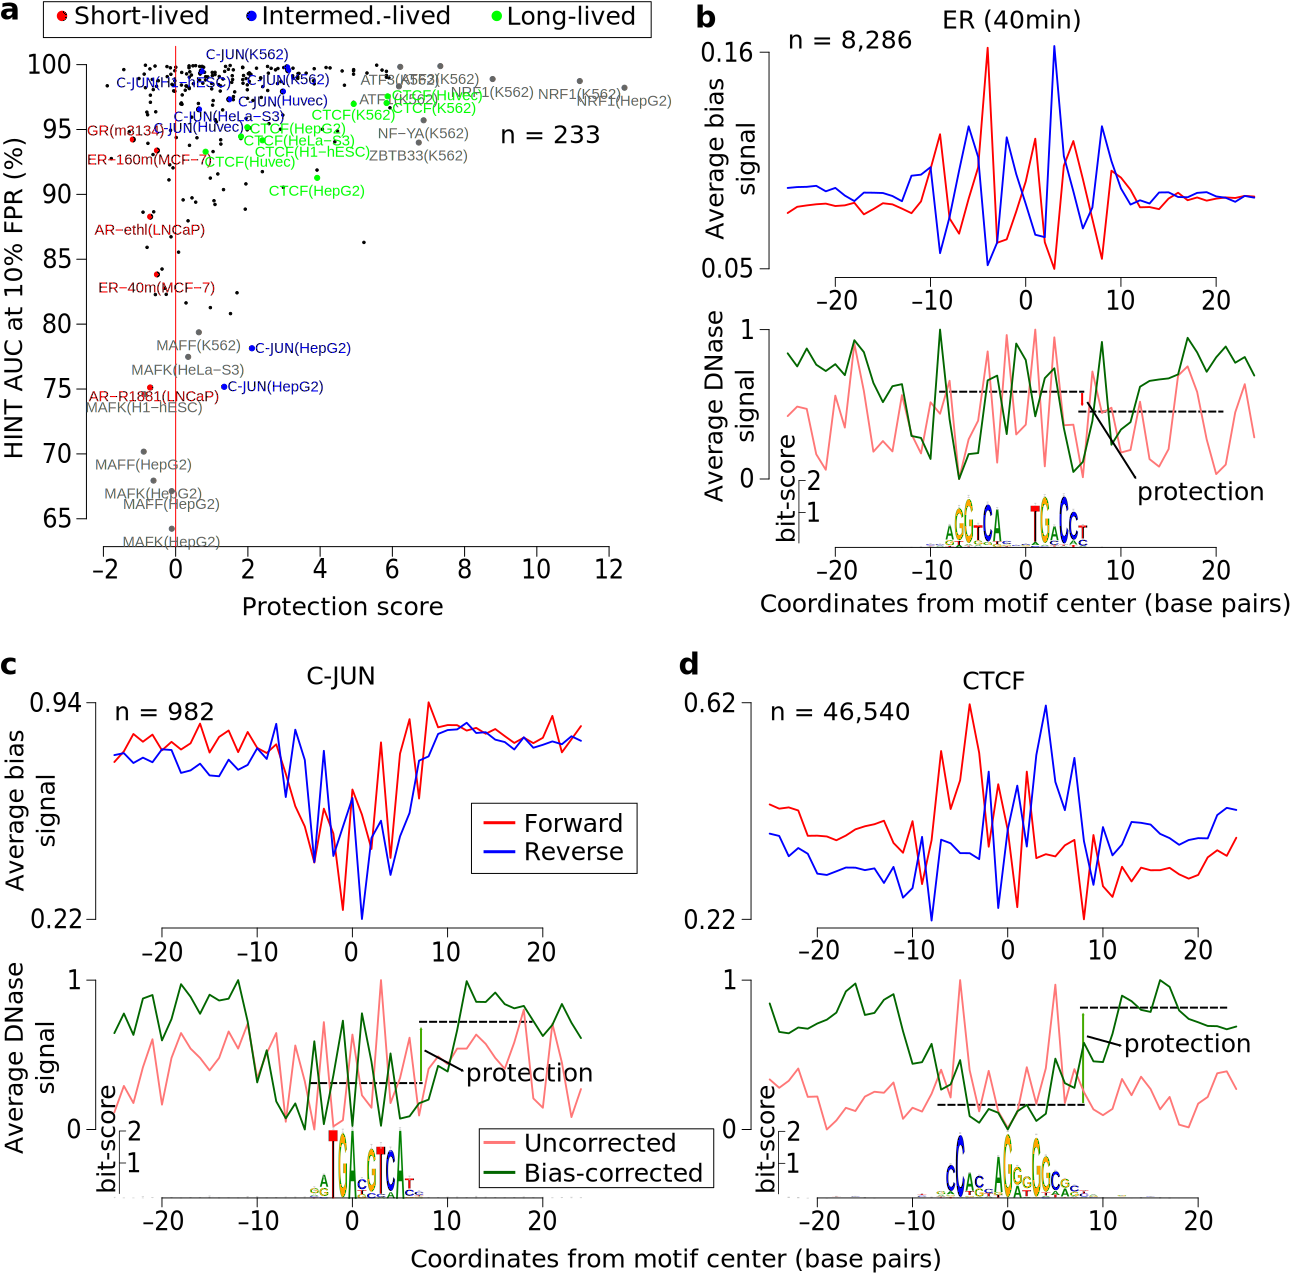
\includegraphics[width=0.99\textwidth]{gusmao_residence_time}
\caption[Impact of transcription factor residence binding time on computational footprinting]{\textbf{Impact of transcription factor residence binding time on computational footprinting.} (\textbf{a}) Scatter plot with the protection score ($x$-axis) \emph{vs} the AUC (at $10\%$ FPR) of HINT ($y$-axis) for the transcription factors from the {\tt Comprehensive Dataset}. We highlight nuclear receptors AR, ER and GR (short residence time, red); C-JUN (intermediate residence time, blue); CTCF (long residence time, green) and other transcription factors with either high ($> 6$) protection score or low ($< 0.8$) AUC values (grey). (\textbf{b}--\textbf{d}) Average bias signal (top) and uncorrected/bias-corrected DNase-seq signal (bottom) for the transcription factors (\textbf{b}) ER, (\textbf{c}) C-JUN and (\textbf{d}) CTCF. Signals in the bottom graph were standardized to be in the interval $[0,1]$. The motif logo represents all underlying DNA sequences centered on the transcription factor binding sites.}
\label{fig:gusmao_residence_time}
\end{figure}






























%%%%%%%%%%%%%%%%%%%%%%%%%%%%%%%%%%%%%%%%%%%%%%%%%%%%%%%%%%%%%%%%%%%%%
% Section: HINT Case Studies -- Identification of Regulatory TFs involved in Different Biological Conditions
%%%%%%%%%%%%%%%%%%%%%%%%%%%%%%%%%%%%%%%%%%%%%%%%%%%%%%%%%%%%%%%%%%%%%
\section{HINT Case Studies -- Identification of Regulatory TFs involved in Different Biological Conditions}
\label{sec:case.studies}

% Introduction
In this chapter we show two case studies in which our computational footprinting method was successfully used to identify key regulatory players on two different biological analyses. Both case studies exhibit a similar experimental workflow. Briefly, we first apply HINT to detect footprint predictions in different cellular conditions. Then, we compare these different cellular conditions to find the transcription factors more likely to be associated with each condition. This common footprint \emph{post hoc} experiment is called ``transcription factor enrichment analysis''. The main goal of the transcription factor enrichment analysis is to identify transcription factors which are more likely to bind in footprints from a particular cell type when compared to other cell type.

% This section
We start this section by describing the transcription factor enrichment analysis, which is necessary to the understanding of the case studies' results (Section~\ref{sec:transcription.factor.enrichment.analysis}). Then we show our analysis on the first case study regarding the identification of key regulatory transcription factors on the differentiation of dendritic cells in mouse (Section~\ref{sec:case.study.dendritic}). The second case study concerns the identification of transcription factors associated to (i.e. binds together with) the NF-$\kappa$B transcription factor, which is a key regulator on the mammalian inflammatory response (Section~\ref{sec:case.study.nfkb}).

%%%%%%%%%%%%%%%%%%%%%%%%%%%%%%%%%%%%%%%%%%%%%%%%%%%%%%%%%%%%%%%%%%%%%
% Section: Transcription Factor Enrichment Analysis
%%%%%%%%%%%%%%%%%%%%%%%%%%%%%%%%%%%%%%%%%%%%%%%%%%%%%%%%%%%%%%%%%%%%%
\subsection{Transcription Factor Enrichment Analysis}
\label{sec:transcription.factor.enrichment.analysis}

% Introduction
The transcription factor enrichment analysis can be divided in two parts: (1) the application of a statistical test, on each cell type or biological condition, to verify if transcription factors bind more than expected by chance at genomic regions of interest (i.e. footprints); and (2) the comparison between the results of the statistical test for all transcription factors between the different cell types or biological conditions being investigated.

% Target vs background genomic region sets
We start by defining two genomic region sets: the target genomic region set and the background genomic region set. The target genomic region set $X = \{ x_1, \cdots, x_n \}$ is composed of the genomic regions associated to the target biological condition being tested (Figure~\ref{fig:gusmao_enrichment_analysis}a). It can be, for instance, footprints identified in a group of differentially expressed genes. The background genomic region set $Y = \{ y_1, \cdots, y_m \}$ (Figure~\ref{fig:gusmao_enrichment_analysis}b) is composed of a collection of random genomic regions throughout the genome. The rationale is that the background genomic region set acts as a ``control'' to which we can compare our target genomic region set against. By comparing the occurrence of putative active transcription factor binding within our target genomic region set $X$ against the background genomic region set $Y$ we can perform a statistical test to assess the enrichment of transcription factors in $X$. For statistical power, the number of background genomic regions $m$ should be at least $10$ times higher than the number of target genomic regions $n$.

% Motif analysis and overlap
After the definition of our target and background genomic region sets, we apply the motif matching algorithm to identify motif-predicted binding sites within these regions (Figure~\ref{fig:gusmao_enrichment_analysis}c). In the analyses presented in this thesis, the motif matching was performed using all the position frequency matrices available from Jaspar~\cite{mathelier2014} and Uniprobe~\cite{robasky2011}. Then, by overlapping the motif-predicted binding sites with the target and background genomic region sets, we create the following statistics for each transcription factor $t$ (Figure~\ref{fig:gusmao_enrichment_analysis}d):

\vspace{0.3cm}
\noindent
$a_t$ -- The number of target genomic regions overlapping at least one MPBS from TF $t$. \vspace{0.2cm} \\
$b_t$ -- The number of target genomic regions which do not overlap any MPBS from TF $t$. \vspace{0.2cm} \\
$c_t$ -- The number of background genomic regions overlapping at least one MPBS from TF $t$. \vspace{0.2cm} \\
$d_t$ -- The number of background genomic regions which do not overlap any MPBS from TF $t$.\\
\vspace{0.3cm}

% Fisher's exact test
Then, we apply the Fisher's exact test on the aforementioned statistics $a_t$, $b_t$, $c_t$ and $d_t$. The null hypothesis is defined as: the proportion transcription factor binding at target genomic regions is not greater than the proportion of transcription factor binding at background genomic regions. Nevertheless, since we test a high number of transcription factors (\approxy$600$ PFMs from Jaspar and Uniprobe) and each one requires a different and independent statistical test, we perform a multiple testing correction. For that, we use the Benjamini and Hochberg method~\cite{benjamini1995} (also known as false discovery rate (FDR) control method). The final result is a list of corrected $p$-values which describes the likelihood of the tested transcription factors to be associated to the target genomic regions in comparison to the background genomic regions.

% Comparison
In possession of the corrected $p$-value list of transcription factor enrichment for all cell types / biological conditions being tested, we search for the transcription factors that presented significant $p$-values ($< 0.05$) in particular cell types / biological conditions. For that, we filter the list of transcription factors for the ones which: (1) present a significant $p$-value in at least one of the conditions tested and (2) present a non significant $p$-value in at least one of the conditions tested. The list of filtered transcription factors are likely to contain the regulators of specific cell types / biological conditions.

% Figure - Transcription factor enrichment analysis
\begin{figure}[h!]
\centering
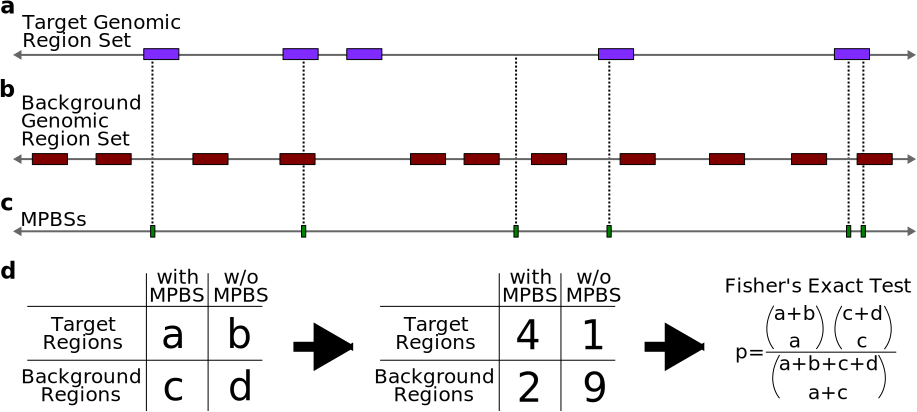
\includegraphics[width=0.99\textwidth]{gusmao_enrichment_analysis}
\caption[Transcription factor enrichment analysis]{\textbf{Transcription factor enrichment analysis.} (\textbf{a}) The target genomic region set is composed of the genomic regions under study. (\textbf{b}) The background genomic region set is composed of ``control'' genomic regions. It can be, for instance, random genomic regions in the same organism's genome. (\textbf{c}) Motif-predicted binding sites (motif-predicted binding sites) are created for a particular transcription factor in which we are interested in evaluating if enriched in the target genomic regions in contrast to the background genomic regions. (\textbf{d}) Based on the overlap between the target genomic region set, the background genomic region set and the motif-predicted binding sites for a particular transcription factor, we create a contingency table and evaluate the Fisher's exact test. The test's $p$-value gives an indication on the enrichment of the transcription factor at the target genomic regions.}
\label{fig:gusmao_enrichment_analysis}
\end{figure}

%%%%%%%%%%%%%%%%%%%%%%%%%%%%%%%%%%%%%%%%%%%%%%%%%%%%%%%%%%%%%%%%%%%%%
% Section: Case Study: Regulatory Network during Differentiation of Dendritic Cells
%%%%%%%%%%%%%%%%%%%%%%%%%%%%%%%%%%%%%%%%%%%%%%%%%%%%%%%%%%%%%%%%%%%%%
\subsection{Case Study: Regulatory Network during Differentiation of Dendritic Cells}
\label{sec:case.study.dendritic}

% Introduction - goals of study
Dendritic cells (DCs) are professional antigen presenting cells that develop from hematopoietic stem cells through successive steps of lineage commitment and differentiation. Multipotent progenitors (MPPs) are committed to common DC progenitors (CDPs), which further differentiate into specific DC subsets: the classical DCs (cDCs) and plasmacytoid DCs (pDCs). The goal of this study is to understand the epigenetic and regulatory circuitry that determines the differentiation of MPPs to CDPs and CDPs to either cDCs or pDCs. Furthermore, it is known that the transcription factor PU.1 is an important factor on the differentiation of DCs (termed master regulator, given the fact that it initiates differentiation events). The understanding of DC differentiation has impact on the further understanding of adaptive immune response.

% Here
In this study, ChIP-seq experiments were performed for several histone modifications, including H3K4me1. With the goal to capture the regulatory landscape of dendritic cell differentiation, we performed a transcription factor enrichment analysis using the footprints predicted with HINT on ChIP-seq for H3K4me1. The transcription factor enrichment analysis was performed using two different subsets of footprints. The H3K4me1 footprints that overlap with the master regulator transcription factor PU.1 ChIP-seq enriched regions (peaks) and the ones that do not overlap with PU.1. This analysis, which is a part of the study performed by Lin et al.~\cite{lin2015}, is presented as a case study for our computational footprinting framework in the next subsections.

%%%%%%%%%%%%%%%%%%%%%%%%%%%%%%%%%%%%%%%%%%%%%%%%%%%%%%%%%%%%%%%%%%%%%
% Section: Computational Footprinting
%%%%%%%%%%%%%%%%%%%%%%%%%%%%%%%%%%%%%%%%%%%%%%%%%%%%%%%%%%%%%%%%%%%%%
\subsubsection{Computational Footprinting}
\label{sec:cs1.computational.footprinting}

% Computational Footprinting
We applied the histone-only HINT model (see ``Histone-only HMM'' in Section~\ref{sec:hmm.topology}) to the H3K4me1 ChIP-seq data. We followed the experimental settings as described in Chapter~\ref{cha:experiments}. Briefly, we extended the H3K4me1 enriched regions by $5,000$ bp to each side and applied our histone-only HMM model trained with H3K4me1 data from random genomic regions. Given the lower resolution of ChIP-seq data and the nature of the probabilistic model, footprints from H3K4me1 tend to span larger regions. Therefore, we further reduced the footprint predictions by considering only $250$ bp to the left (downstream) and right (upstream) of its center.

% Motif enrichment analysis
After the computational footprinting on H3K4me1 data, we used the footprint predictions to perform a transcription factor enrichment analysis. We performed two different analyses. The first, considered H3K4me1 footprints that overlaps ChIP-seq peaks from the transcription factor PU.1 as the target genomic regions set. The second considered as target genomic regions set, the H3K4me1 footprints that do not overlap PU.1 binding sites. These two definitions of target genomic region sets were used for data on the four different cells being analyzed: MPPs, CDPs, cDCs and pDCs. In all tests, the size of the background genomic region sets were $100$ times higher than the size of the target genomic region sets.

%%%%%%%%%%%%%%%%%%%%%%%%%%%%%%%%%%%%%%%%%%%%%%%%%%%%%%%%%%%%%%%%%%%%%
% Section: Results
%%%%%%%%%%%%%%%%%%%%%%%%%%%%%%%%%%%%%%%%%%%%%%%%%%%%%%%%%%%%%%%%%%%%%
\subsubsection{Results}
\label{sec:cs1.results}

% Intersection
The Figure~\ref{fig:lin_footprint_enrichment_s8}a shows the overlap between H3K4me1 footprints and PU.1 ChIP-seq enriched regions (peaks). We can observe different levels of overlap. A higher overlap was found on more specialized cells (cDC; \approxy$68\%$ of H3K4me1 footprints overlap with PU.1 peaks) in contrast to more plastic cells (MPP; \approxy$23\%$ of H3K4me1 footprints overlap with PU.1 peak). These results are consistent with gene expression information obtained with RNA-seq analyses, which shows higher expression of PU.1 in cDC than MPP cell types~\cite{lin2015}.

% Two enrichment analysis - PU.1 and H3K4me1 footprints
We present here three transcription factor enrichment analysis results, corresponding to experiments that searched for enriched transcription factors: (1) only in PU.1 peaks (Figure~\ref{fig:lin_footprint_enrichment_s8}b); (2) in H3K4me1 footprints that overlap PU.1 peaks (Figure~\ref{fig:lin_footprint_enrichment_s8}c) and (3) in H3K4me1 footprints that did not overlap PU.1 peaks (Figure~\ref{fig:lin_footprint_enrichment_s8}d). The $p$-values from the transcription factor enrichment analyses are presented as a heatmap. The enrichment is represented in a gray to blue scale. A gray heatmap entry represent no enrichment ($p$-value $> 0.05$) for the transcription factor represented in the row at the cell type represented in the column. A blue heatmap entry represents evidence of enrichment ($p$-value $< 0.05$). Enriched transcription factors were separated in different clusters (numbered I to VI) given their enrichment in different cells. 

% Results TFs
We were able to detect many transcription factors involved in the differentiation of transcription factors. In MPP we observed the binding of the pioneer PU.1 alongside evidence of KLF4 and RUNX1. The AP1-like transcription factors (FOS and JUN) and some IRF factors (IRF2, IRF4 and IRF5) appear to be cDC-specific. This means that these factors might have some role on the differentiation from CDP to cDC cell type. On the other hand, TCF factors (TCF3 and TCF4), EGR1 and KLF4 appear to play a role in the differentiation from CDP to pDC cell type.

% Results main
Interestingly, the transcription factor enrichment analysis performed in H3K4me1 footprints have captured most of the PU.1-only enrichment analysis. Furthermore, the H3K4me1 footprint analyses recovered two transcription factors (CEBPB and BHLHE40; marked in red in Figure~\ref{fig:lin_footprint_enrichment_s8}c--d) which were not found by the PU.1-only enrichment analysis.

% Figure - Dendritic cells footprint enrichment analysis results
\begin{figure}[h!]
\centering
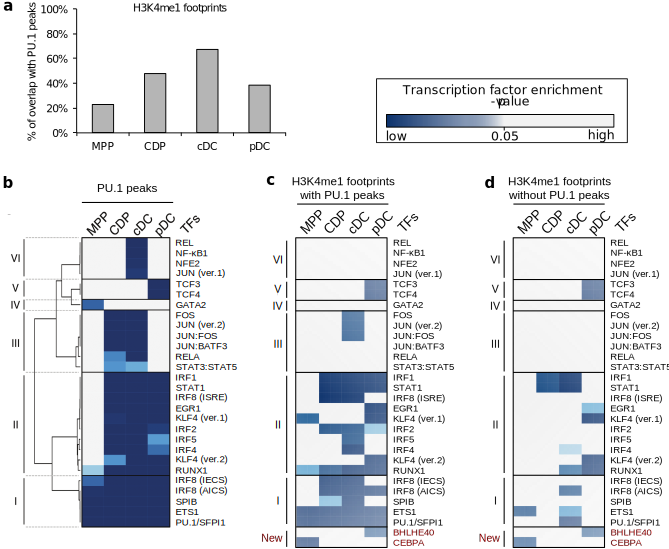
\includegraphics[width=0.99\textwidth]{lin_footprint_enrichment_s8}
\caption[Dendritic cells footprint enrichment analysis results]{\textbf{Dendritic cells footprint enrichment analysis results.} (\textbf{a}) The overlap between dendritic cell's master regulator transcription factor PU.1 ChIP-seq enriched regions with H3K4me1 footprints in the context of dendritic cell differentiation. (\textbf{b}--\textbf{d}) Heatmap depicts the enrichment of transcription factor motifs in MPP, CDP, cDC and pDC based on: (\textbf{b}) PU.1 peaks, (\textbf{c}) H3K4me1 footprints overlapping PU.1 peaks and (\textbf{d}) H3K4me1 footprints not overlapping PU.1 peaks. The $p$-values are plotted and color-coded using a continuous spectrum from gray ($p$-value > 0.05) to blue ($p$-value < 0.05). We mark in red the transcription factors which were found to be enriched in the H3K4me1 footprint analyses and not in the PU.1-only analysis. \emph{Source: Lin et al.}\cite{lin2015} (modified to fit thesis format and/or clarify key points).}
\label{fig:lin_footprint_enrichment_s8}
\end{figure}

% Conclusion
The results presented here demonstrate the power of computational footprinting coupled with the transcription factor enrichment analysis to increase the sensitivity of biological analyses. The H3K4me1 footprints represent regulatory regions and were shown to have a high overlap (\approxy$80\%$) with open chromatin regions. The H3K4me1 footprint predictions were used to search for transcription factors which act in conjunction with PU.1 master regulator or independently from the PU.1 master regulator. Such results, combined with other experimental data and knowledge from previous studies, were used to devise a regulatory network on the differentiation of dendritic cells. The complete results of these experiments can be found in Lin et al.~\cite{lin2015}.

%%%%%%%%%%%%%%%%%%%%%%%%%%%%%%%%%%%%%%%%%%%%%%%%%%%%%%%%%%%%%%%%%%%%%
% Section: Case Study: Multimodal Role of NF-kB during Intermmediate-Early Inflammatory Response
%%%%%%%%%%%%%%%%%%%%%%%%%%%%%%%%%%%%%%%%%%%%%%%%%%%%%%%%%%%%%%%%%%%%%
\subsection{Case Study: Multimodal Role of NF-$\kappa$B during Intermmediate-Early Inflammatory Response}
\label{sec:case.study.nfkb}

% Introduction - goals of study
Tumor necrosis factor alpha (TNF$\alpha$) acutely remodels the cell’s transcriptional program, but our understanding of how the activation of proinflammatory genes is achieved at the expense of the ongoing transcriptional program is far from complete. The transcription factor NF-$\kappa$B, the main driver of the inflammatory response, predominantly ``hijacks'' the regulatory machinery of the cell by binding already-active enhancers, more than half of which do not carry NF-$\kappa$B recognition motifs. The study performed by Kolovos et al.~\cite{kolovos2016} present evidence for a multimodal role of NF-$\kappa$B that satisfies the need for both transcriptional activation and suppression, and is linked with changes in the higher-order structure of regulated loci.

% Here
One of the analysis performed in Kolovos et al.~\cite{kolovos2016} regards a transcription factor enrichment analysis to understand the transcription factors associated to NF-$\kappa$B in regions that: either carry the NF-$\kappa$B DNA recognition motif or do not exhibit such motif. The analysis was performed on human Huvec cell type (umbilical vein/vascular endothelium). This analysis, which is a part of the study performed by Kolovos et al.~\cite{kolovos2016}, is presented as a case study for our computational footprinting framework in the next subsections.

%%%%%%%%%%%%%%%%%%%%%%%%%%%%%%%%%%%%%%%%%%%%%%%%%%%%%%%%%%%%%%%%%%%%%
% Section: Computational Footprinting
%%%%%%%%%%%%%%%%%%%%%%%%%%%%%%%%%%%%%%%%%%%%%%%%%%%%%%%%%%%%%%%%%%%%%
\subsubsection{Computational Footprinting}
\label{sec:cs2.computational.footprinting}

% Data
DNase-seq raw reads from Huvecs were obtained from ENCODE~\cite{encode2012}. The data is available in GEO with accession number GSM816646. The short reads from the DNase-seq experiment were aligned to the human reference genome~\cite{encode2012} using Bowtie~\cite{langmead2012}. To identify the DNase I hypersensitivity regions (DNase-seq enriched regions), the software F-seq~\cite{boyle2008b} was applied to the aligned reads (using the procedure described in Section~\ref{sec:dnaseseq.enriched.regions}).

% Computational Footprinting
Then, we applied the DNase-only HINT model (see ``DNase-only HMM'' in Section~\ref{sec:hmm.topology}) to the DNase-seq data. We followed the experimental settings as described in Chapter~\ref{cha:experiments}. Briefly, we extended the DNase I hypersensitivity regions by $5,000$ bp to each side and applied our DNase-only HMM model trained with DNase-seq data from the Huvec experiments presented in this thesis.

% Motif Enrichment Analysis
The resulting footprint predictions from the DNase-only HINT were separated in two categories. The footprint predictions that overlaps NF-$\kappa$B ChIP-seq enriched regions~\cite{papantonis2012} that: (1) carries the canonical NF-$\kappa$B motif and (2) do not carry such motif. Then we performed a transcription factor enrichment analysis in these two different conditions, considering the footprint predictions as our target genomic region set. The size of the background genomic region sets were $100$ times higher than the size of the target genomic region sets.

%%%%%%%%%%%%%%%%%%%%%%%%%%%%%%%%%%%%%%%%%%%%%%%%%%%%%%%%%%%%%%%%%%%%%
% Section: Results
%%%%%%%%%%%%%%%%%%%%%%%%%%%%%%%%%%%%%%%%%%%%%%%%%%%%%%%%%%%%%%%%%%%%%
\subsubsection{Results}
\label{sec:cs2.results}

% Introduction
NF-$\kappa$B binding predominantly occurs at already-active (upon inflammation stimuli) distal regulatory regions called enhancers. These are mostly intragenic, display little overlap with CTCF-bound sites, and half carry the canonical motif or remain bound by NF-$\kappa$B at $60$ min after inflammatory stimulation. To obtain a more precise view of NF-$\kappa$B binding choices, we performed a transcription factor enrichment analysis on DNase-seq footprints. The analysis consists on comparing two different genomic region sets: (1) NF-$\kappa$B ChIP-seq enriched regions (peaks) at enhancer regions with the canonical NF-$\kappa$B motif and (2) NF-$\kappa$B ChIP-seq enriched regions (peaks) at enhancer regions without the canonical NF-$\kappa$B motif.

% Heatmap
The result of the transcription factor enrichment analysis can be seen in Figure~\ref{fig:kolovos_footprint_enrichment_2c}. We exhibit a heatmap that combines the two conditions tested. The color code is a gradient from blue (transcription factors enriched in NF-$\kappa$B peaks with motif) to white (no enrichment) to red (transcription factors enriched in NF-$\kappa$B peaks without motif).

% Results main
As expected, REL-like transcription factors (REL, RELA and NF-$\kappa$B1) are enriched in the NF-$\kappa$B peaks with canonical motif. Furthermore, the transcription factors KLF4, KLF7, ZNF281 and EGR1 appear to be significantly enriched in these regions. Among these factors, there are the TNF$\alpha$-induced REL, RELA, NF-$\kappa$B1, KLF7 and EGR1. On the other hand, we observe that the transcription factors  are significantly associated to NF-$\kappa$B-binding enhancer regions without the canonical NF-$\kappa$B motif. The only TNF$\alpha$-repressed transcription factor that appeared in our enrichment analysis -- SOX17 -- appears to be slightly associated to the regions without NF-$\kappa$B motif. The mechanisms behind these associated transcription factors and human inflammatory response are further explored in Kolovos et al.~\cite{kolovos2016}.

% Further evidence
In summary, the analysis have shown that REL-like transcription factors (RELA and NF-$\kappa$B1) are markedly enriched at the NF-$\kappa$B peaks with canonical motif; whereas AP1-like transcription factors (JUN and FOS) appear to be enriched at the NF-$\kappa$B peaks without canonical motif. Further analyses show that the footprint enrichment analysis prediction is backed by ENCODE~\cite{encode2012} ChIP-seq data from Huvecs, where co-binding of NF-$\kappa$B and JUN/FOS (and to a lesser extent GATA2) was most prominent at enhancers without NF-$\kappa$B recognition sites.

% Figure - Huvec cells footprint enrichment analysis results
\begin{figure}[h!]
\centering
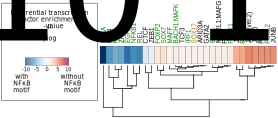
\includegraphics[width=0.99\textwidth]{kolovos_footprint_enrichment_2c}
\caption[Huvec cells footprint enrichment analysis results]{\textbf{Huvec cells footprint enrichment analysis results.} Heatmap showing the transcription factor enrichment analysis results at Huvec enhancer regions that overlap the footprints predicted with the DNase-only HINT model. The heatmap represents enrichment between ChIP-seq enriched regions with (blue) and without the canonical NF-$\kappa$B motif (red). Transcription factors induced or repressed by the inflammatory response factor TNF$\alpha$ are demarcated green and yellow, respectively. \emph{Source: Kolovos et al.}\cite{kolovos2016} (modified to fit thesis format and/or clarify key points).}
\label{fig:kolovos_footprint_enrichment_2c}
\end{figure}

% Conclusion
In contrast with the previous case study (Section~\ref{sec:case.study.dendritic}), where different cell types were being analyzed for the putative regulatory elements within their open chromatin regions; the analysis presented in this case study was based on two conditions which differed only in the presence/absence of the NF-$\kappa$B motif. In this case, the usage of DNase-seq alleviates much of the noise from intervening unbound sequence. The results presented in this section, combined with other experimental data, were used to understand the mechanisms behind hijacked enhancers and the regulatory role of NF-$\kappa$B in the human inflammatory mechanism. The complete results of these experiments can be found in Kolovos et al.~\cite{kolovos2016}.














































%%%%%%%%%%%%%%%%%%%%%%%%%%%%%%%%%%%%%%%%%%%%%%%%%%%%%%%%%%%%%%%%%%%%%
% Section: Discussion
%%%%%%%%%%%%%%%%%%%%%%%%%%%%%%%%%%%%%%%%%%%%%%%%%%%%%%%%%%%%%%%%%%%%%
\section{Discussion}
\label{sec:discussion.5}

% TODO

% Introduction
In this chapter we provided an investigation on state-of-the-art computational footprinting methods. We show results regarding parameter selection, selection of optimal ranking criteria, biological experimental bias correction, issues regarding the transcription factor residence time, examples of post-hoc analyses such as \emph{de novo} motif finding and transcription factor enrichment. Furthermore, a comprehensive comparative study on a significant number of computational footprinting methods was performed.

% Conclusion
In conclusion, the assessment of computational footprinting methods is a demanding task, both computationally and technically. We have created a fair and reproducible benchmarking data set for evaluation of protein-DNA binding using two validation approaches: using ChIP-seq and using gene expression. Although the rationales of the ChIP-seq and gene expression evaluation procedures are, in principle, very different, we observed a high agreement between their respective ranking of methods. This is evidence that this study provides a robust map of the accuracy of state-of-the-art computational footprinting methods.


